\documentclass[cjk,slidestop,compress,mathserif,blue]{beamer}
%\documentclass[cjk,slidestop,handout,compress,mathserif,blue]{beamer}	%打印PPT用,handout(讲义)可去掉过渡效果,如\pause引起的多页显示,为打印时节省纸张
%dvipdfm选项是关键,否则编译统统通不过
%beamer的颜色选项定义的是导航条和标题的颜色(即关键词structure的颜色)

%%%%%%%%%%%%%%%%仅限于XeTeX可使用的宏包%%%%%%%%%%%%%%%%%%%%%%%%%%%%
\usepackage{fontspec,xunicode,xltxtra,beamerthemesplit}
%\usepackage{beamerthemesplit}
\usepackage{handoutWithNotes}		%(讲义)在打印PPT的时候会留出给每一页做注释的部分
\usepackage{xeCJK}
\setCJKmainfont[BoldFont=黑体, ItalicFont=楷体, BoldItalicFont=仿宋]{黑体}
%\setsansfont[Mapping=tex-text]{Adobe 黑体 Std}
%如果装了Adobe Acrobat,可在font.conf中配置Adobe字体的路径以使用其中文字体
%也可直接使用系统中的中文字体如SimSun,SimHei,微软雅黑 等
%原来beamer用的字体是sans family;注意Mapping的大小写,不能写错

\usepackage{listings} 
\lstset{language=Matlab}%代码语言使用的是matlab 
\lstset{breaklines}%自动将长的代码行换行排版 
\lstset{extendedchars=false}%解决代码跨页时,章节标\dots

%%%%%%%%   确定标题和导航条结构的框架     %%%%%%%%%%%%
\usepackage{beamerthemeshadow}                       %
%\usepackage{beamerthemeclassic}%导航条色与背景色一致%
%%%%%%%%%%%%%%%%%%%%%%%%%%%%%%%%%%%%%%%%%%%%%%%%%%%%%%
\setbeamerfont{roman title}{size={}}
%\usepackage{CJK} % CJK 中文支持                                  %
\usepackage{amsmath,amsthm,amsfonts,amssymb,bm}
\usepackage{mathrsfs}
\usepackage{xcolor}                                        %使用默认允许使用颜色
\usepackage{hyperref} 
\usepackage{graphicx}
\usepackage{subfigure}           %图片跨页
\usepackage{animate}		 %插入动画
\usepackage{caption}
\captionsetup{font=footnotesize}

\usepackage{verbatim}			%Verbatim 宏包重新实现了 Verbatim 环境,并且提供一个命令可以导入一个 ASCII 文件到文档中
\usepackage{multirow}
% A LATEX package for embedding interactive Adobe Flash (SWF) and 3D files (Adobe U3D & PRC) as well as video and sound files or streams (FLV, MP4/H.246, MP3) into PDF documents with Adobe Reader-9
\usepackage[dvipdfmx]{movie15_dvipdfmx} %插入视频之一
%\usepackage{media9}			%插入视频之一
%\usepackage{multimedia}			%插入视频之一
%\usepackage{handoutWithNotes}		%(讲义)在打印PPT的时候会留出给每一页做注释的部分
%\pgfpagesuselayout{1 on 1 with notes landscape}[a4paper,border shrink=5mm]

%\usepackage[numbers,sort&compress]{natbib} %紧密排列             %
\usepackage[sectionbib]{chapterbib}        %每章节单独参考文献   %
\usepackage{hypernat}                                                                         %
\setbeamertemplate{bibliography item}[text] %参考文献前标注[]
%\usepackage[dvipdfm,bookmarksopen=true,pdfstartview=FitH,CJKbookmarks]{hyperref}		%
\hypersetup{bookmarksnumbered,colorlinks,linkcolor=brown,citecolor=blue,urlcolor=red}         %
%参考文献含有超链接引用时需要下列宏包,注意与natbib有冲突        %
%\usepackage[dvipdfm]{hyperref}                                  %
%\usepackage{hypernat}                                           %
\newcommand{\upcite}[1]{\hspace{0ex}\textsuperscript{\cite{#1}}} %

%\useoutertheme{smoothbars}
\useinnertheme[shadow=true]{rounded}
\usetheme{Berkeley}                                          %主题式样
%\usetheme{Luebeck}

\usecolortheme{lily}                                        %颜色主题式样

\usefonttheme{professionalfonts}                           %字体主题样式宏包

%\beamertemplatetransparentcoveredhigh                      %使所有被隐藏的文本高度透明
\beamertemplatetransparentcovereddynamicmedium             %使所有被隐藏的文本完全透明,动态,动态的范围很小
\mode<presentation>
%\beamersetaveragebackground{gray}                          %设置背景颜色(单一色) 
\beamertemplateshadingbackground{green!10}{red!5}         %设置背景颜色(渐变色)

\graphicspath{{/home/jiangjun/Documents/Latex_Beamer/}}                            %
%i放置单位logo
%\logo{\includegraphics[width=1.6cm,height=0.35cm]{Figures_Peking-Opera/BCC_logo-1.png}}	%简单设置logo

%\pgfdeclareimage[width=3.5cm]{logoname}{Figures_Peking-Opera/BCC_logo-1.png}		%logo置于左侧微调
%\logo{\pgfuseimage{logoname}{\vspace{0.2cm}\hspace*{-2.0cm}}}

%在指定位置精确放置logo
\usepackage{tikz}
\usepackage{beamerfoils}
\usepackage{pgf}
\logo{\pgfputat{\pgfxy(10.68,0.00)}{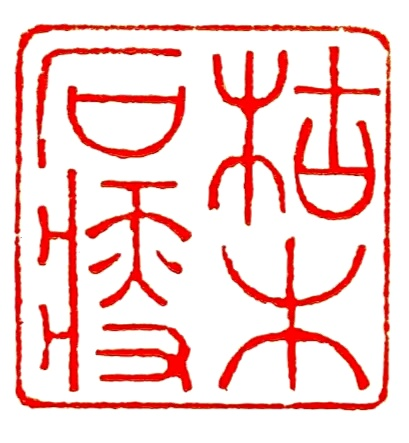
\includegraphics[height=1.20cm,viewport=0 15 400 430,clip]{Figures_Peking-Opera/seal_Jiang-2.jpg}}
     %\pgfputat{\pgfxy(10.817,-0.218)}{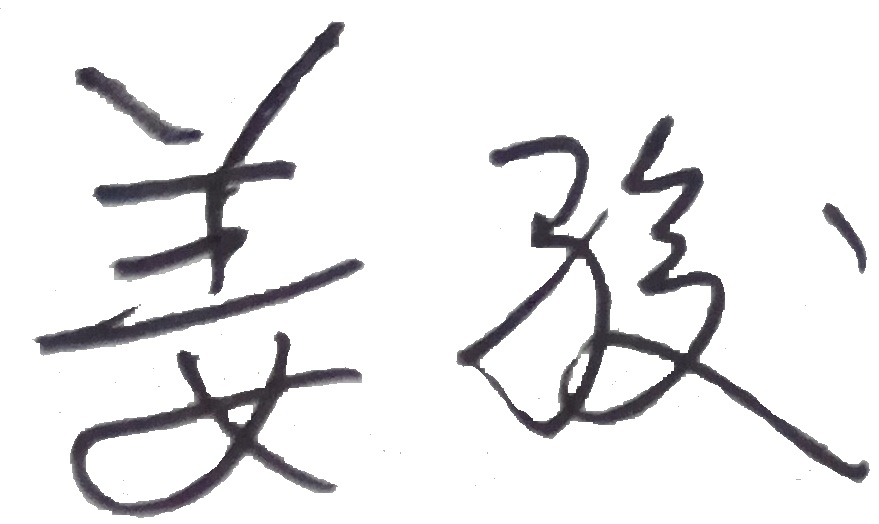
\includegraphics[height=0.47cm,viewport=20 0 670 350,clip]{Figures_Peking-Opera/signature_Jiang_new.jpg}}
}
%\logo{\pgfputat{\pgfxy(11.68,0.252)}{
\includegraphics[height=0.89cm,viewport=0 15 810 800,clip]{Figures_Peking-Opera/seal_Jiang-new.jpg}}\pgfputat{\pgfxy(10.762,-0.218)}{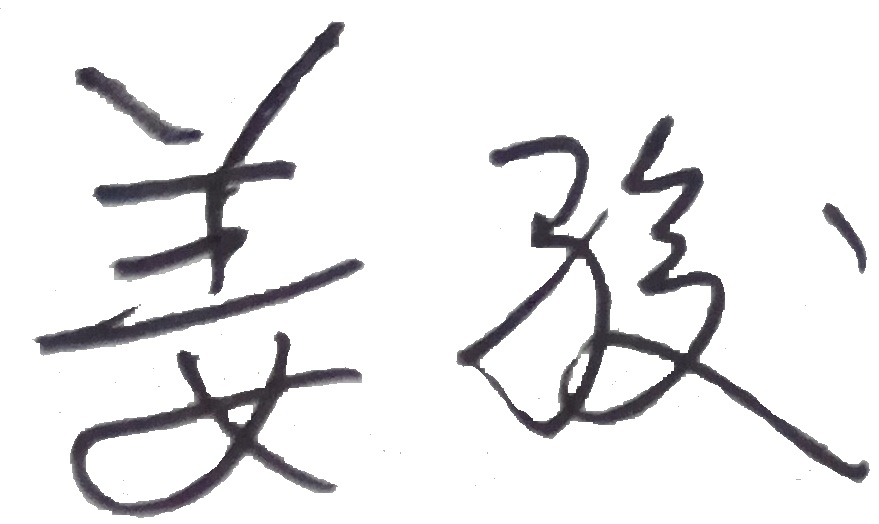
\includegraphics[height=0.49cm,viewport=20 0 670 350,clip]{Figures_Peking-Opera/signature_Jiang_new.jpg}}}
%\logo{\pgfputat{\pgfxy(11.68,0.252)}{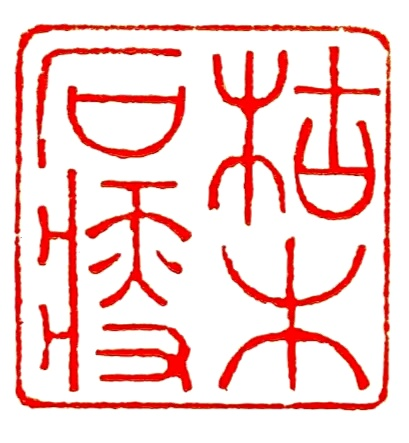
\includegraphics[height=0.90cm,viewport=0 15 400 430,clip]{Figures_Peking-Opera/seal_Jiang-2.jpg}}\pgfputat{\pgfxy(10.817,-0.218)}{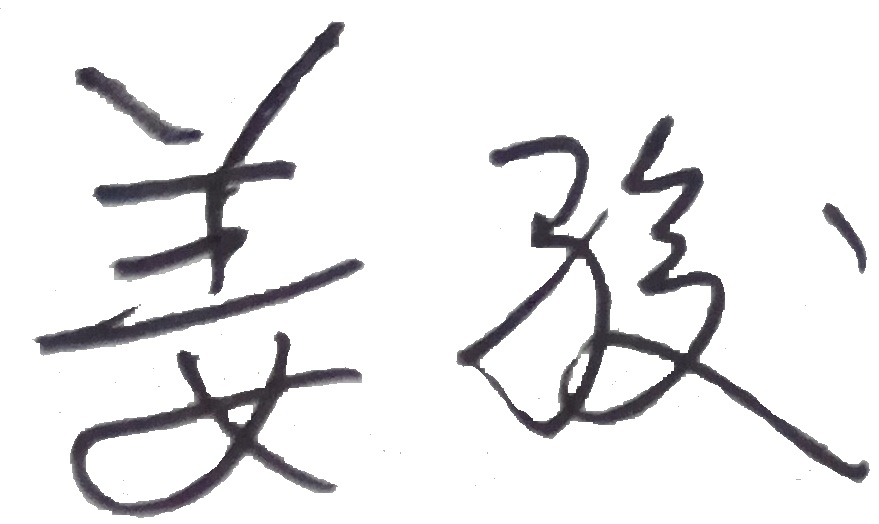
\includegraphics[height=0.47cm,viewport=20 0 670 350,clip]{Figures_Peking-Opera/signature_Jiang_new.jpg}}}
%\logo{\pgfputat{\pgfxy(11.68,0.15)}{\includegraphics[height=1.0cm,viewport=0 0 140 120,clip]{Figures_Peking-Opera/BCC_logo-1.png}}\pgfputat{\pgfxy(10.508,-0.22)}{\includegraphics[height=0.369cm,viewport=140 0 540 120,clip]{Figures_Peking-Opera/BCC_logo-1.png}}}
%\MyLogo{
%	\pgfputat{\pgfxy(-50,-50)}{\pgfbox[right,base]{\includegraphics[height=1cm]{Figures_Peking-Opera/BCC_logo-1.png}}}

%logo作为背景放置
%\setbeamertemplate{background}{
%	\pgfputat{\pgfxy(6.5,-0.5)}{\pgfbox[left,top]{\pgfimage[height=1.1cm]{Figures_Peking-Opera/BCC_logo-1.png}}}}

%\logo{}									%不显示logo

\begin{document}
%\begin{CJK*}{GBK}{song}
%\begin{CJK*}{GBK}{kai}
%beamer下不能用\songyi、\zihao等命令!
%\graphicspath{Figures_Peking-Opera/}

%-------------------------------PPT Title-------------------------------------
\title{如是我闻\\——戏迷眼中的“网事”}
%-----------------------------------------------------------------------------

%----------------------------Author & Date------------------------------------
\author[\textrm{Jun\_Jiang}]{姜~骏\inst{}
%\vskip -20pt 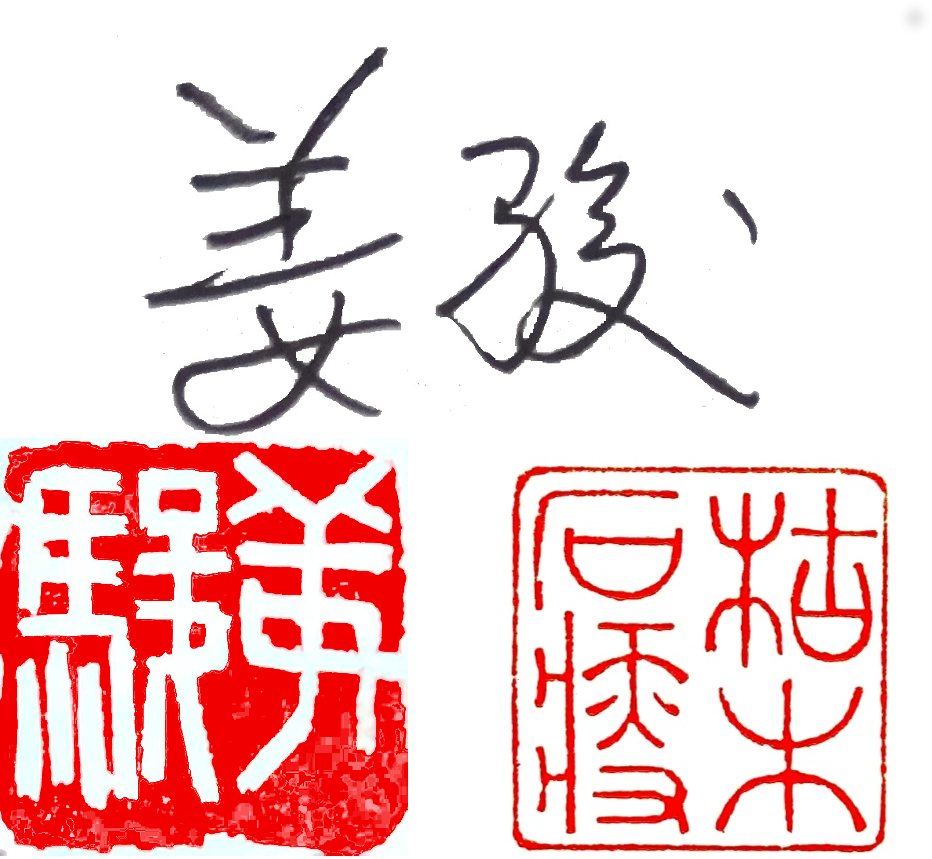
\includegraphics[scale=0.03]{Figures_Peking-Opera/signature-seal_Jiang-1.png} % 加入个人名章 
%\vskip 2pt 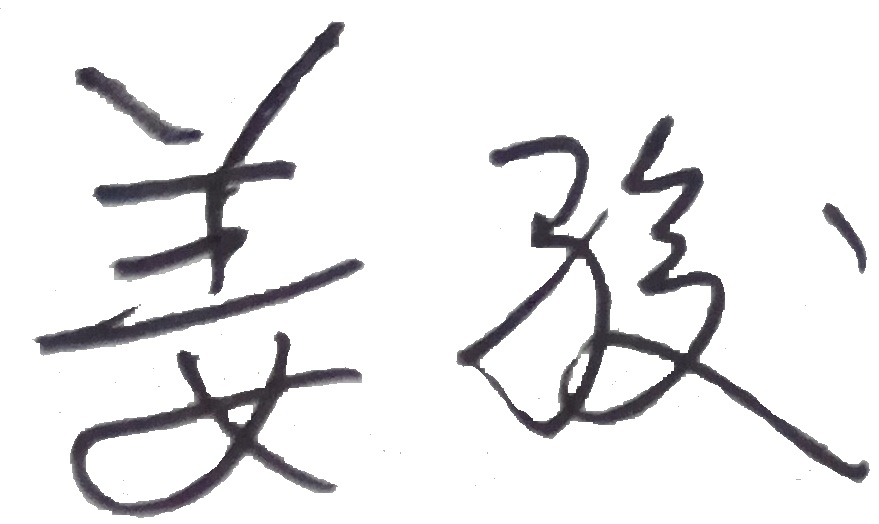
\includegraphics[scale=0.06]{Figures_Peking-Opera/signature_Jiang_new.jpg} % 加入个人签名 
%\vskip -20pt 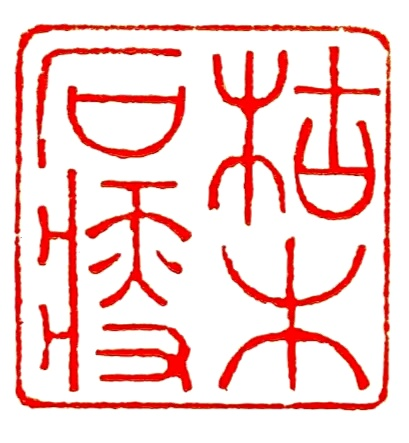
\includegraphics[scale=0.11]{Figures_Peking-Opera/seal_Jiang-2.jpg} % 加入个人闲章 
} %[]{} (optional, use only with lots of authors)
% - Give the names in the same order as the appear in the paper.
% - Use the \inst{?} command only if the authors have different
%   affiliation.
%\institute[BCC]{\inst{}%
 \vskip -30pt %北京市计算中心}
\date[\today] % (optional, should be abbreviation of conference name)
{	{\fontsize{6.2pt}{4.2pt}\selectfont{\textcolor{blue}{E-mail:~}\url{czjiangjun@yeah.cn}}}
\vskip 10 pt {\fontsize{8.2pt}{6.2pt}\selectfont{%报告地点   %清华大学\;\;物理系   
\vskip 5 pt \textrm{2022.04.22}}}
}

% - Either use conference name or its abbreviation
% - Not really information to the audience, more for people (including
%   yourself) who are reading the slides online

\subject{TEST-2}
% This is only inserted into the PDF information catalog. Can be left
% out.
\frame[allowframebreaks]
{
%	\frametitle{\fontsize{9.5pt}{5.2pt}\selectfont{\textcolor{orange}{“高通量并发式材料计算算法与软件”年度检查}}}
\titlepage
}
%-----------------------------------------------------------------------------

\logo{}
%------------------------------------------------------------------------------列出全文 outline ---------------------------------------------------------------------------------
\section*{}
\frame[allowframebreaks]
{
  \frametitle{Outline}
%  \frametitle{\textcolor{mycolor}{\secname}}
  \tableofcontents%[current,currentsection,currentsubsection]
}
%在每个section之前列出全部Outline
%类似的在每个subsection之前列出全部Outline是\AtBeginSubsection[]
\AtBeginSection[]
{
  \frame<handout:0>%[allowframebreaks]%讲义(handout)不显示 <handout:0> 讲义显示 <handout:1> / %beamer不显示 <beamer:0> beamer显示 <beamer:1>	
  {
    \frametitle{Outline}
%全部Outline中,本部分加亮
    \tableofcontents[current,currentsection]
  }
}

%------------------------------------------------------------------------------PPT main Body------------------------------------------------------------------------------------
\small
%\frame
%{
%	\frametitle{引言}
%	2000年左右,随着第一个互联网高峰的到来,戏曲艺术的传播也从传统的广播、电视媒体走向网络。
%}
\section{交流:~校园\rm{BBS}-公众门户网}
\frame
{
	\frametitle{校园京剧社团与论坛:~北大京昆社}
\begin{figure}[h!]
\centering
\vspace{-0.1in}
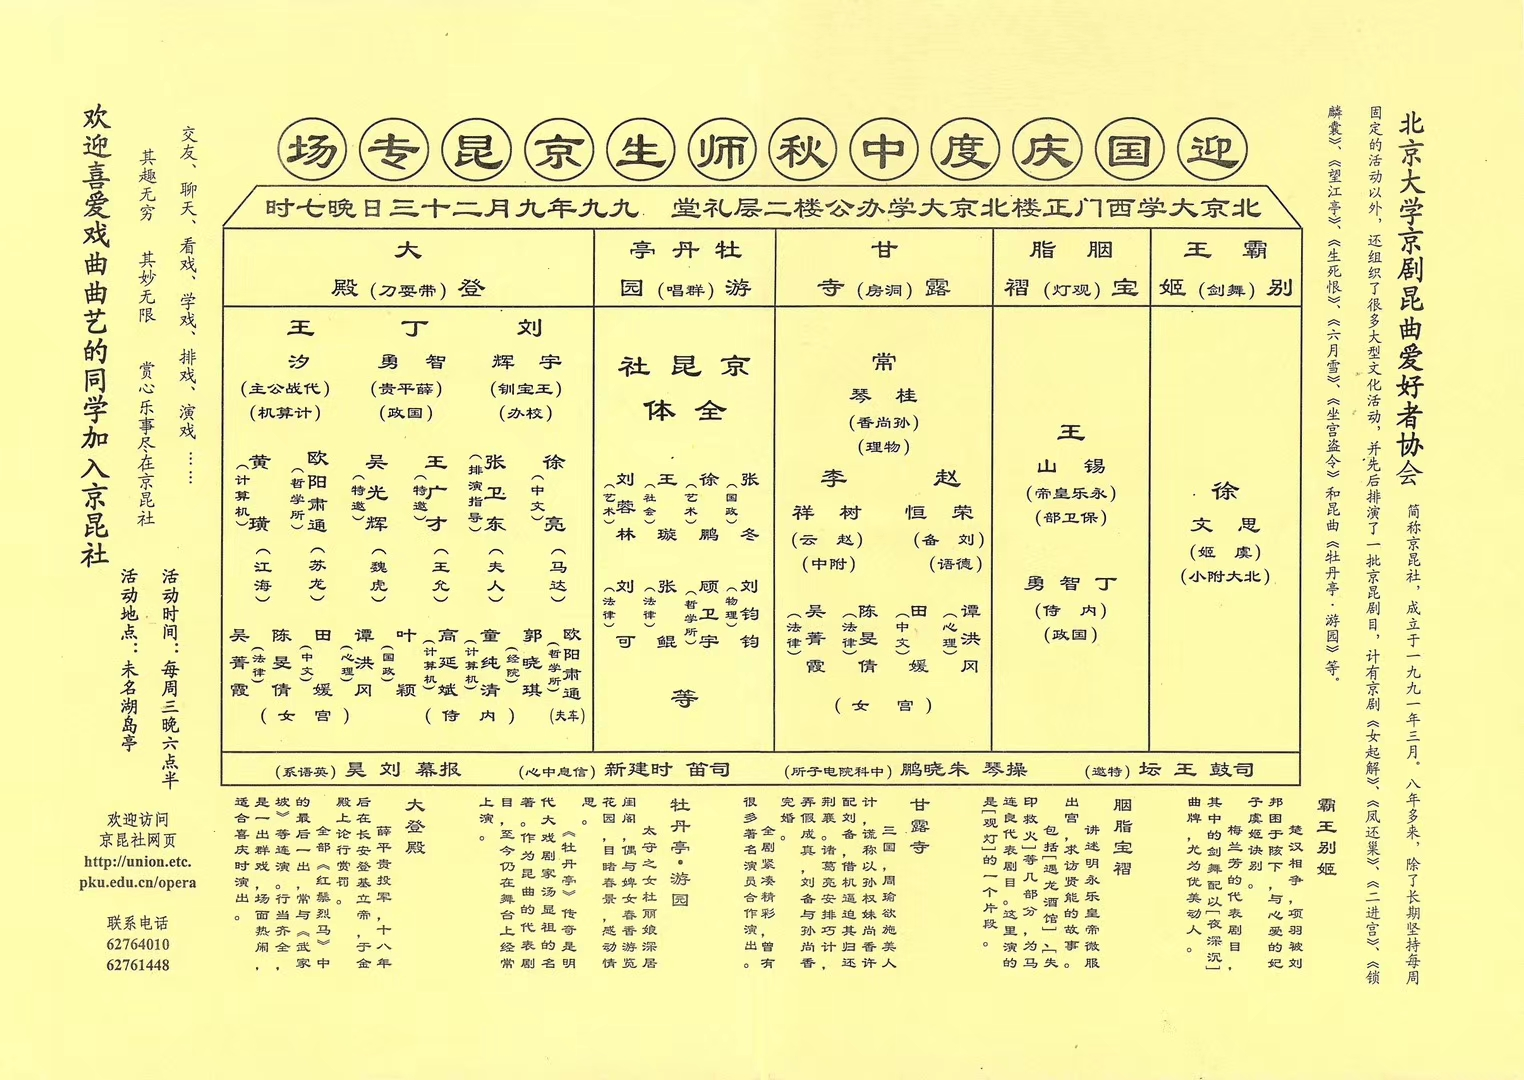
\includegraphics[height=0.70\textwidth,width=0.95\textwidth,clip]{Figures_Peking-Opera/PekOpe_PKU-1.jpg}
\label{PKU-1}
\end{figure}
}

\frame
{
	\frametitle{校园京剧社团与论坛:~北大京昆社}
\begin{figure}[h!]
\centering
\vspace{-0.2in}
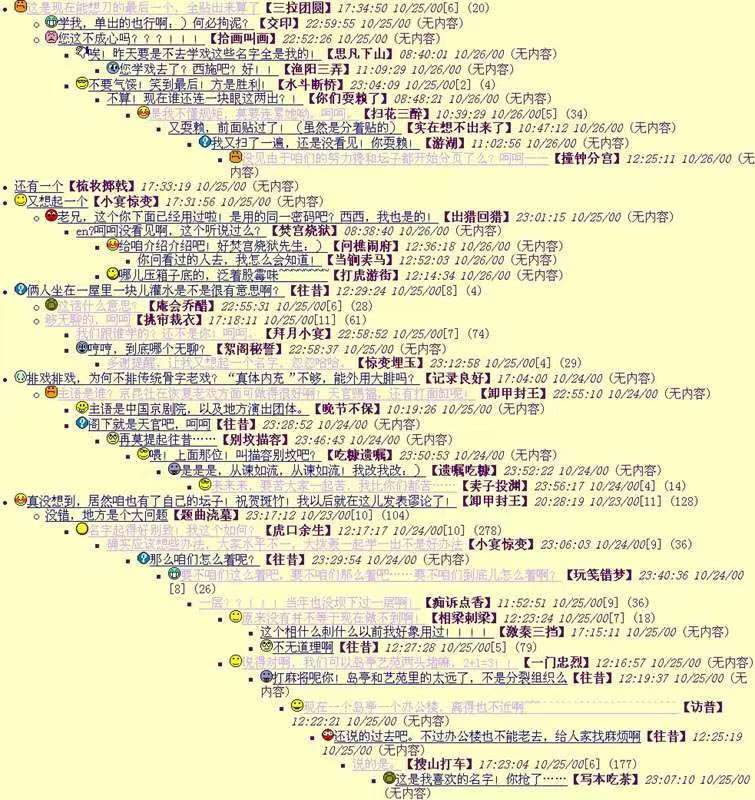
\includegraphics[height=0.75\textwidth,width=0.70\textwidth,clip]{Figures_Peking-Opera/PekOpe_PKU-2.jpg}
\label{PKU-2}
\end{figure}
}

\frame
{
	\frametitle{校园京剧社团与论坛:~北大京昆社}
\begin{figure}[h!]
\centering
\vspace{-0.3in}
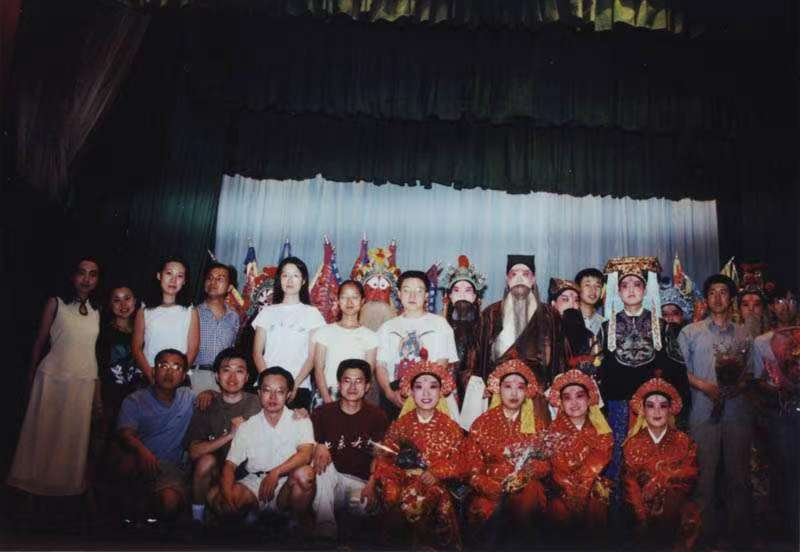
\includegraphics[height=0.70\textwidth,width=1.00\textwidth,clip]{Figures_Peking-Opera/PekOpe_PKU-3.jpg}
\label{PKU-3}
\end{figure}
}

\frame
{
	\frametitle{校园京剧社团与论坛:~清华京剧队}
\begin{figure}[h!]
\centering
\vspace{-0.3in}
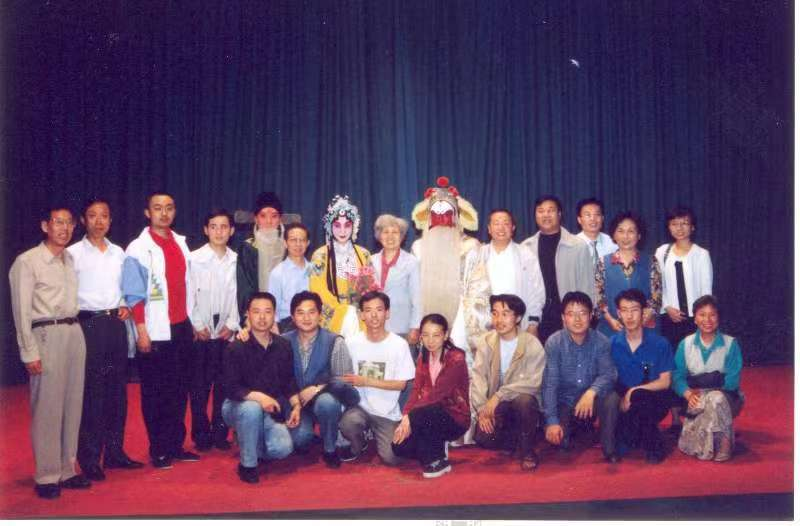
\includegraphics[height=0.70\textwidth,width=1.00\textwidth,clip]{Figures_Peking-Opera/PekOpe_THU-1.jpg}
\label{THU-1}
\end{figure}
}

\frame
{
	\frametitle{校园京剧社团与论坛:~清华京剧队}
\begin{figure}[h!]
\centering
\vspace{-0.3in}
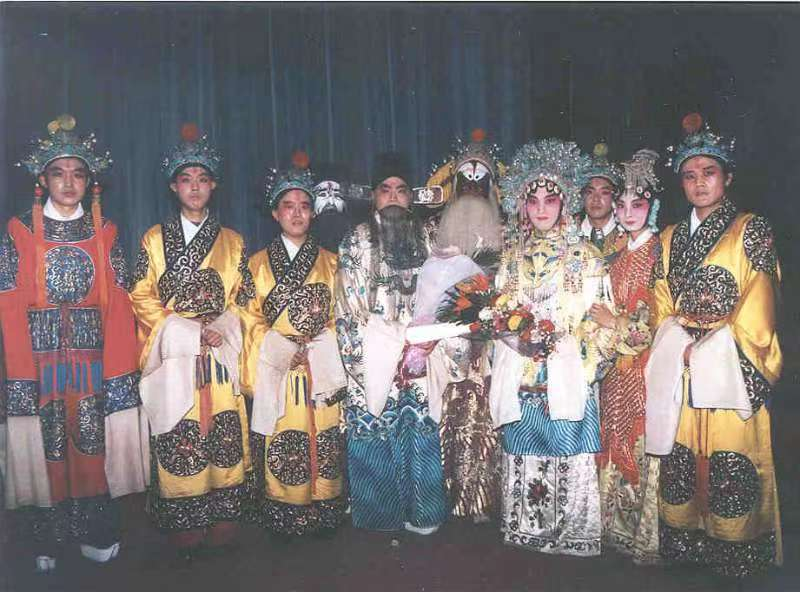
\includegraphics[height=0.70\textwidth,width=1.00\textwidth,clip]{Figures_Peking-Opera/PekOpe_THU-2.jpg}
\label{THU-2}
\end{figure}
}

\frame
{
	\frametitle{校园京剧社团与论坛:~清华京剧队}
\begin{figure}[h!]
\centering
\vspace{-0.2in}
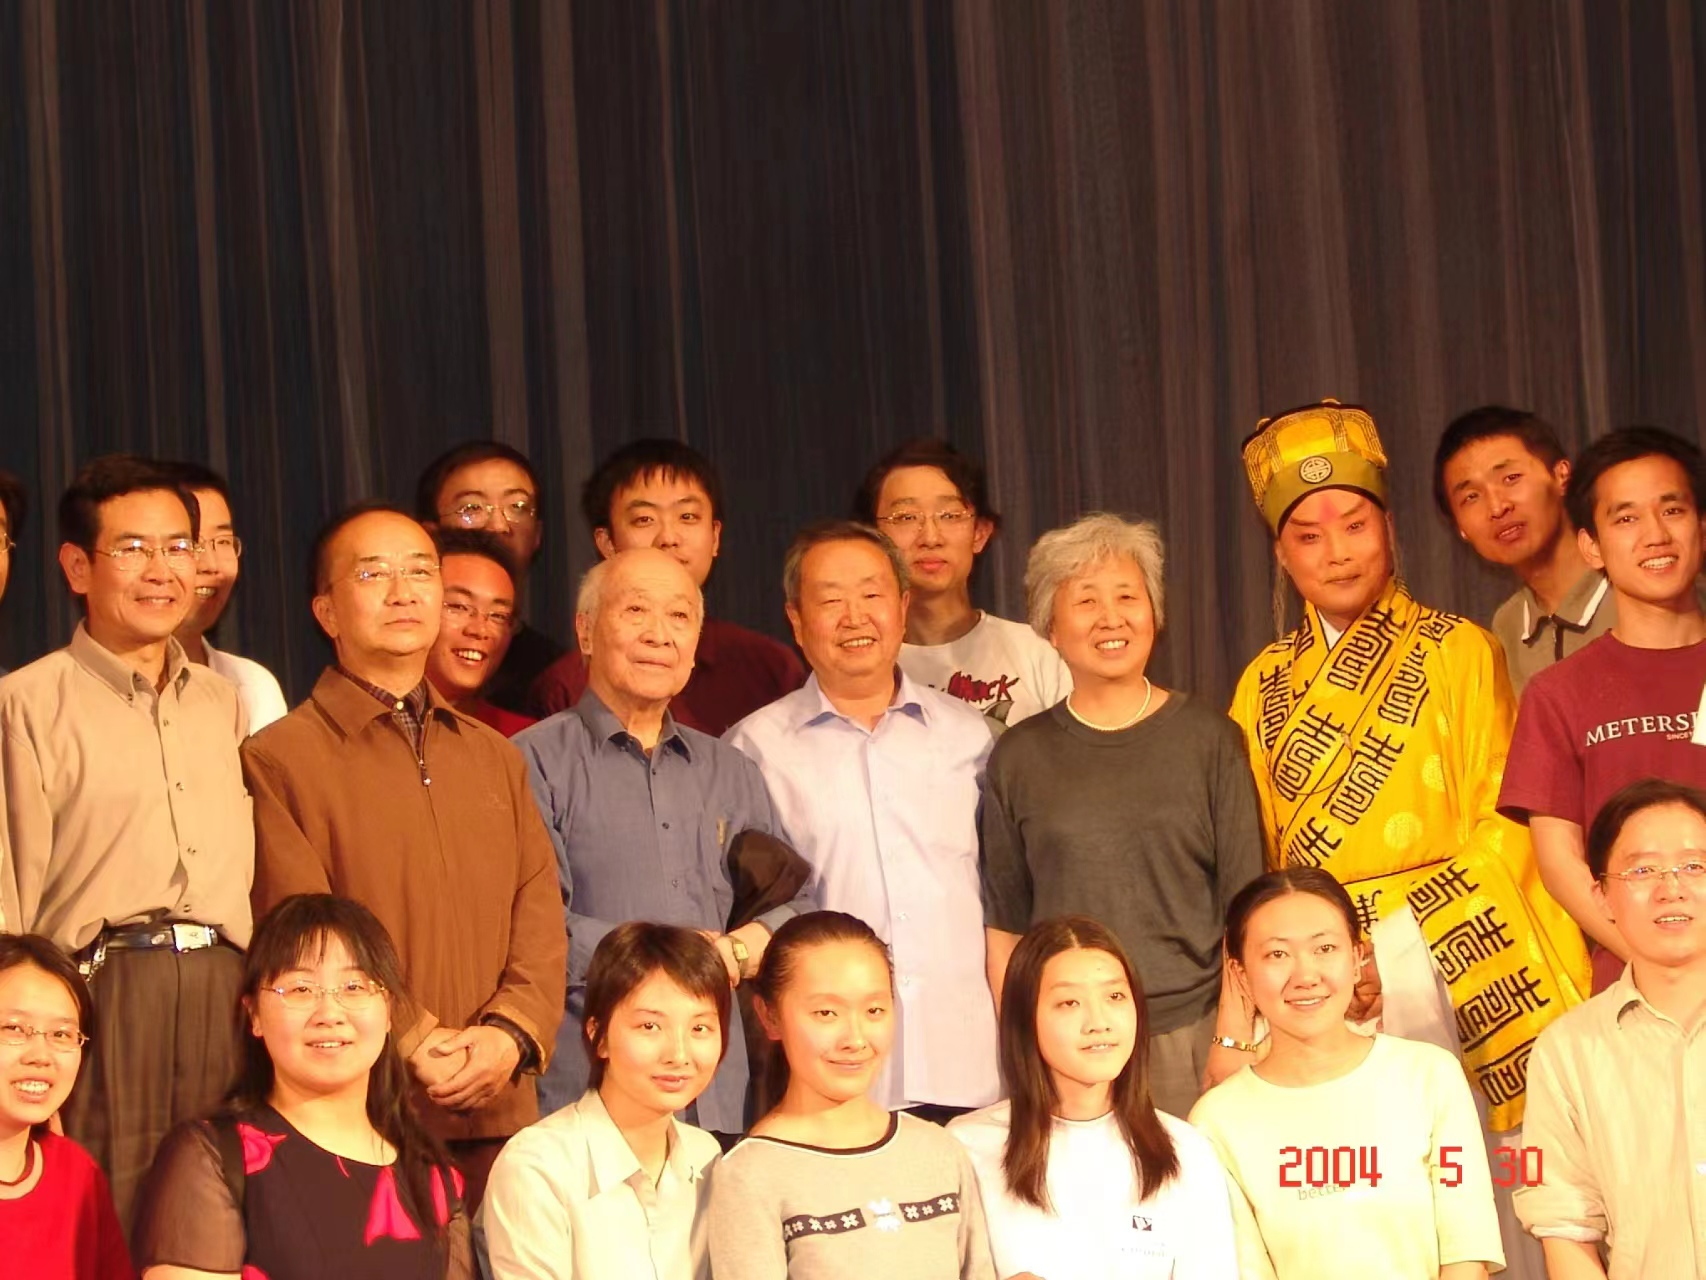
\includegraphics[height=0.70\textwidth,width=1.00\textwidth,clip]{Figures_Peking-Opera/PekOpe_THU-3.jpg}
\label{THU-3}
\end{figure}
}

\frame
{
	\frametitle{校园京剧社团与论坛:~清华京剧队}
\centering
\vspace{-0.15in}
%------------------------------------直-接-插-入-文-件--------------------------------------------------------------------------------------
%\textcolor{red}{\textbf{直接插入文件}}:
\fontsize{4.2pt}{3.2pt}\selectfont{
\verbatiminput{Figures_Peking-Opera/PekOpe_Shuimu.txt} %为保险:~选用文件名绝对路径
}
}

\frame
{
	\frametitle{各大高校的\rm{BBS}中的戏曲板块}
各大高校的\textrm{BBS}几乎都有戏曲版,参与话题的基本以本校的在校学生为主,主题呈现地方特色,但内容丰俭不一
	\begin{itemize}
   		\setlength{\itemsep}{15pt}
		\item 复旦的“日月光华”\textrm{BBS}(昆曲为主)
		\item 西安交大“兵马俑”\textrm{BBS}(侧重秦腔)
		\item 浙大“缥缈云水间”\textrm{BBS}(越剧为主)
		\item 科学院“科苑星空”\textrm{BBS},等等
		\item “一塌糊涂”\textrm{BBS}的\textrm{Drama}版是为数不多的由多个高校网友参与管理和戏曲讨论的开放平台
	\end{itemize}
}

\frame
{
	\frametitle{“一塌糊涂\rm{BBS}”:~跨域校园的论坛}
\begin{figure}[h!]
\centering
\vspace{-0.2in}
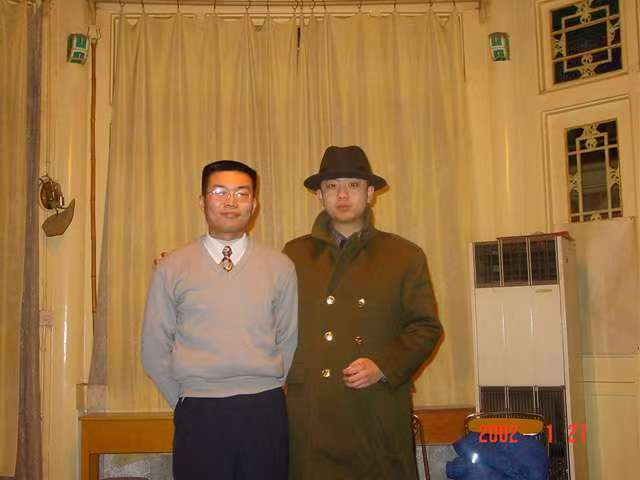
\includegraphics[height=0.70\textwidth,width=0.90\textwidth,clip]{Figures_Peking-Opera/PekOpe_Hutu-1.jpg}
\label{THU}
\end{figure}
}

\frame
{
	\frametitle{《绝版赏析》及其网站}
	电视专题节目《绝版赏析》开播于2001年,开播阶段主要邀请京剧耆宿与名家介绍京剧老唱片为主要形式,后变更为戏曲史事、掌故访谈,辅以唱片。主要由柴俊为先生负责
\begin{figure}[h!]
\centering
\vspace{-0.05in}
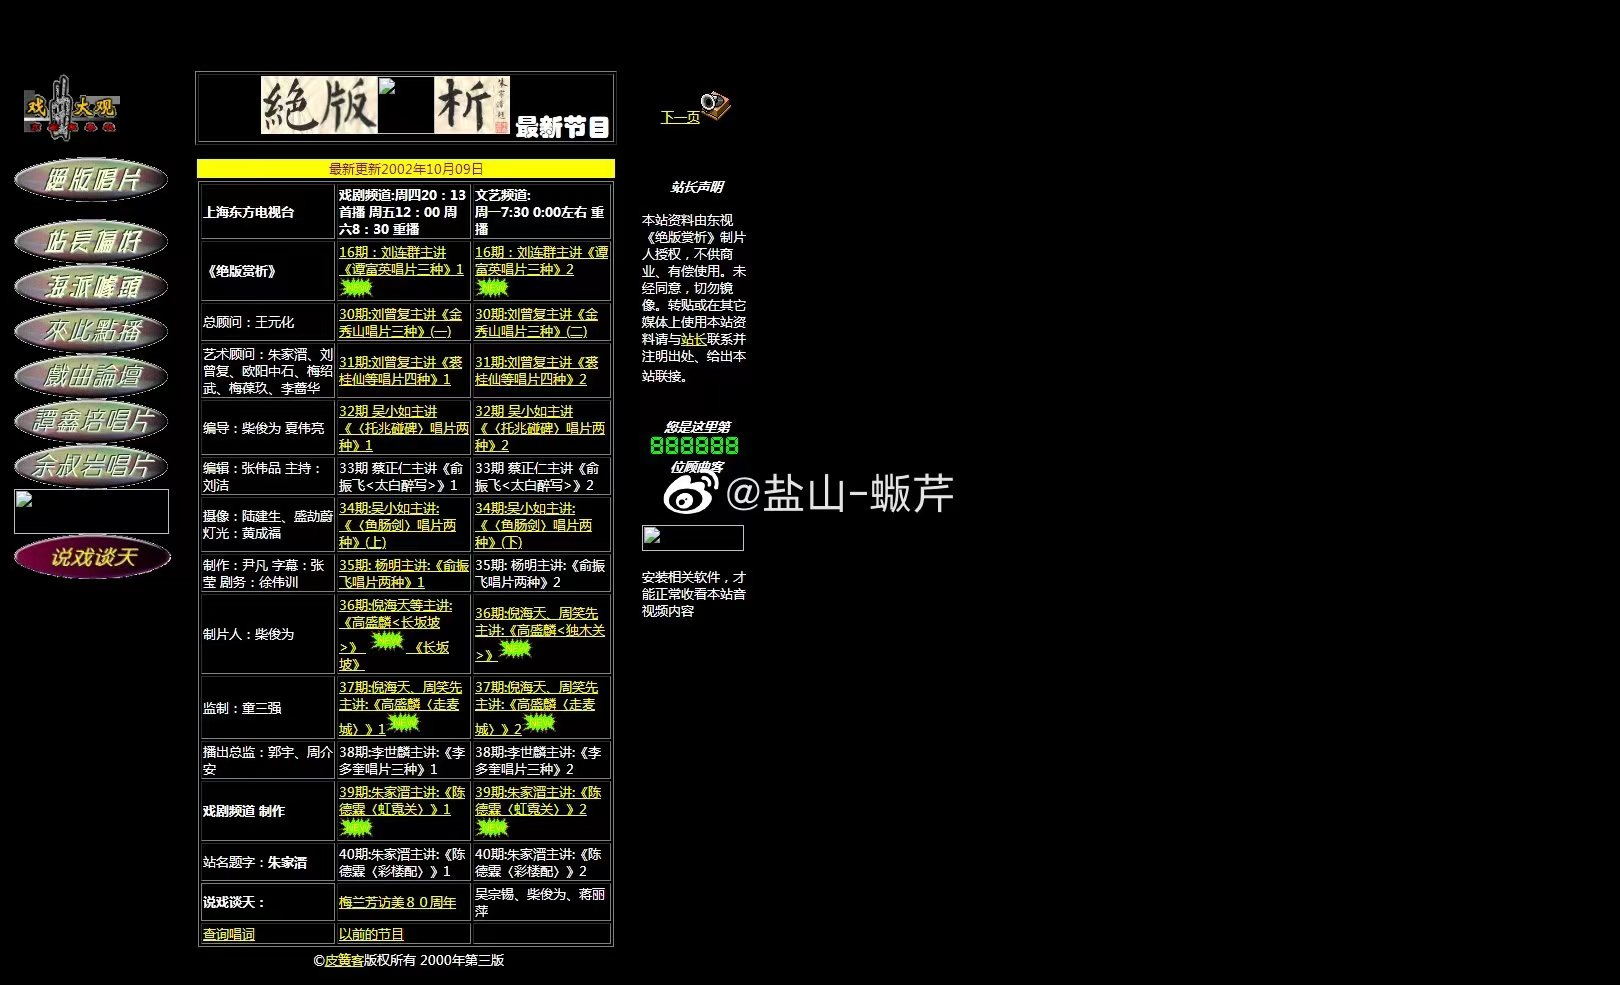
\includegraphics[height=0.55\textwidth,width=0.90\textwidth,clip]{Figures_Peking-Opera/PekOpe_Jueban.jpg}
\label{Jueban}
\end{figure}
}

\frame
{
	\frametitle{咚咚锵和“中国京剧论坛”}
\begin{figure}[h!]
\centering
\vspace{-0.2in}
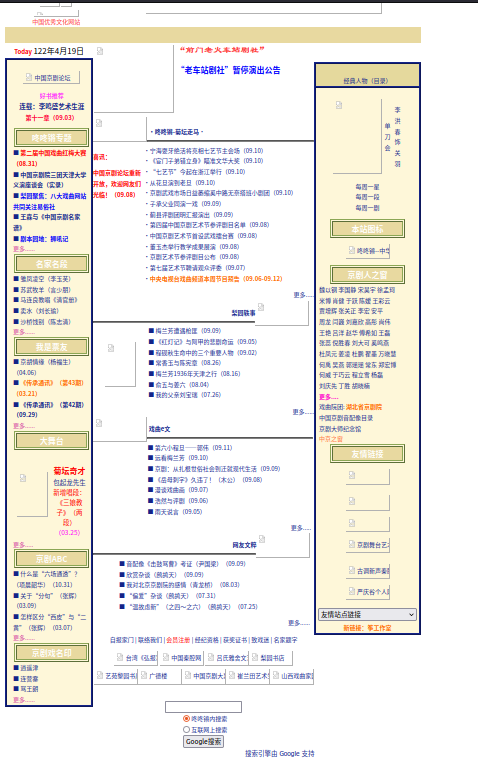
\includegraphics[height=0.8\textwidth,width=0.5\textwidth,clip]{Figures_Peking-Opera/PekOpe_Dongdongqiang.png}
\label{ChnOpe-1}
\end{figure}
}

\frame
{
	\frametitle{咚咚锵和“中国京剧论坛”}
	咚咚锵是“红豆少主”开办的戏曲新闻综合类门户网站,其管理的“中国京剧论坛”是戏迷讨论交流——当然还佐以吵架和骂战——的重要阵地
\begin{figure}[h!]
\centering
\vspace{-0.15in}
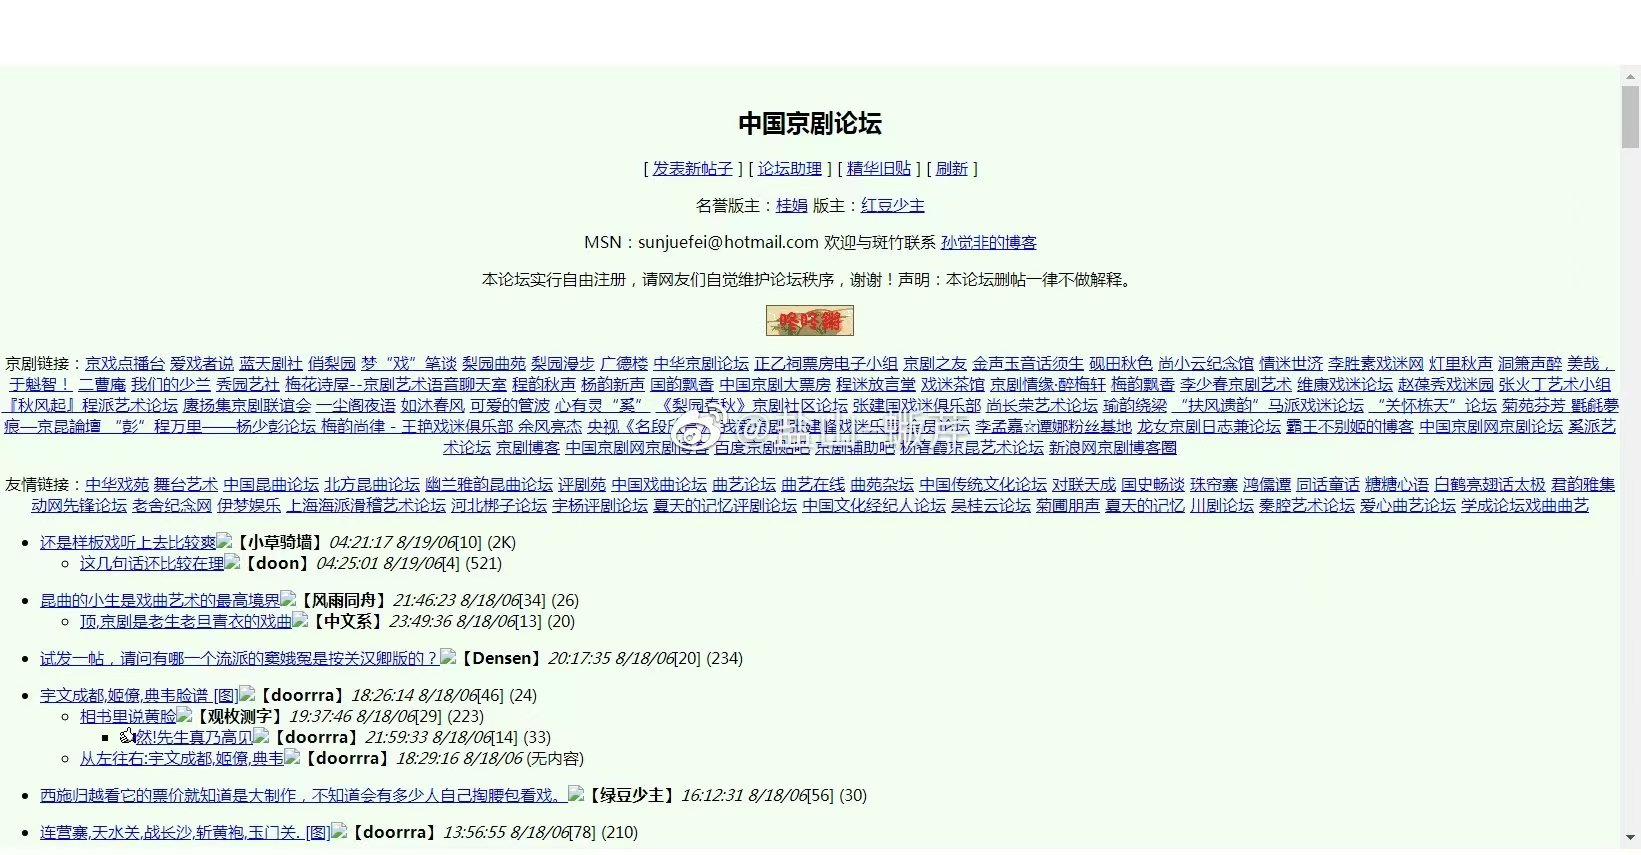
\includegraphics[height=0.55\textwidth,width=1.00\textwidth,clip]{Figures_Peking-Opera/PekOpe_ChnOpe.jpg}
\label{ChnOpe-2}
\end{figure}
}

\frame
{
	\frametitle{时代国粹}
\begin{figure}[h!]
\centering
\vspace{-0.2in}
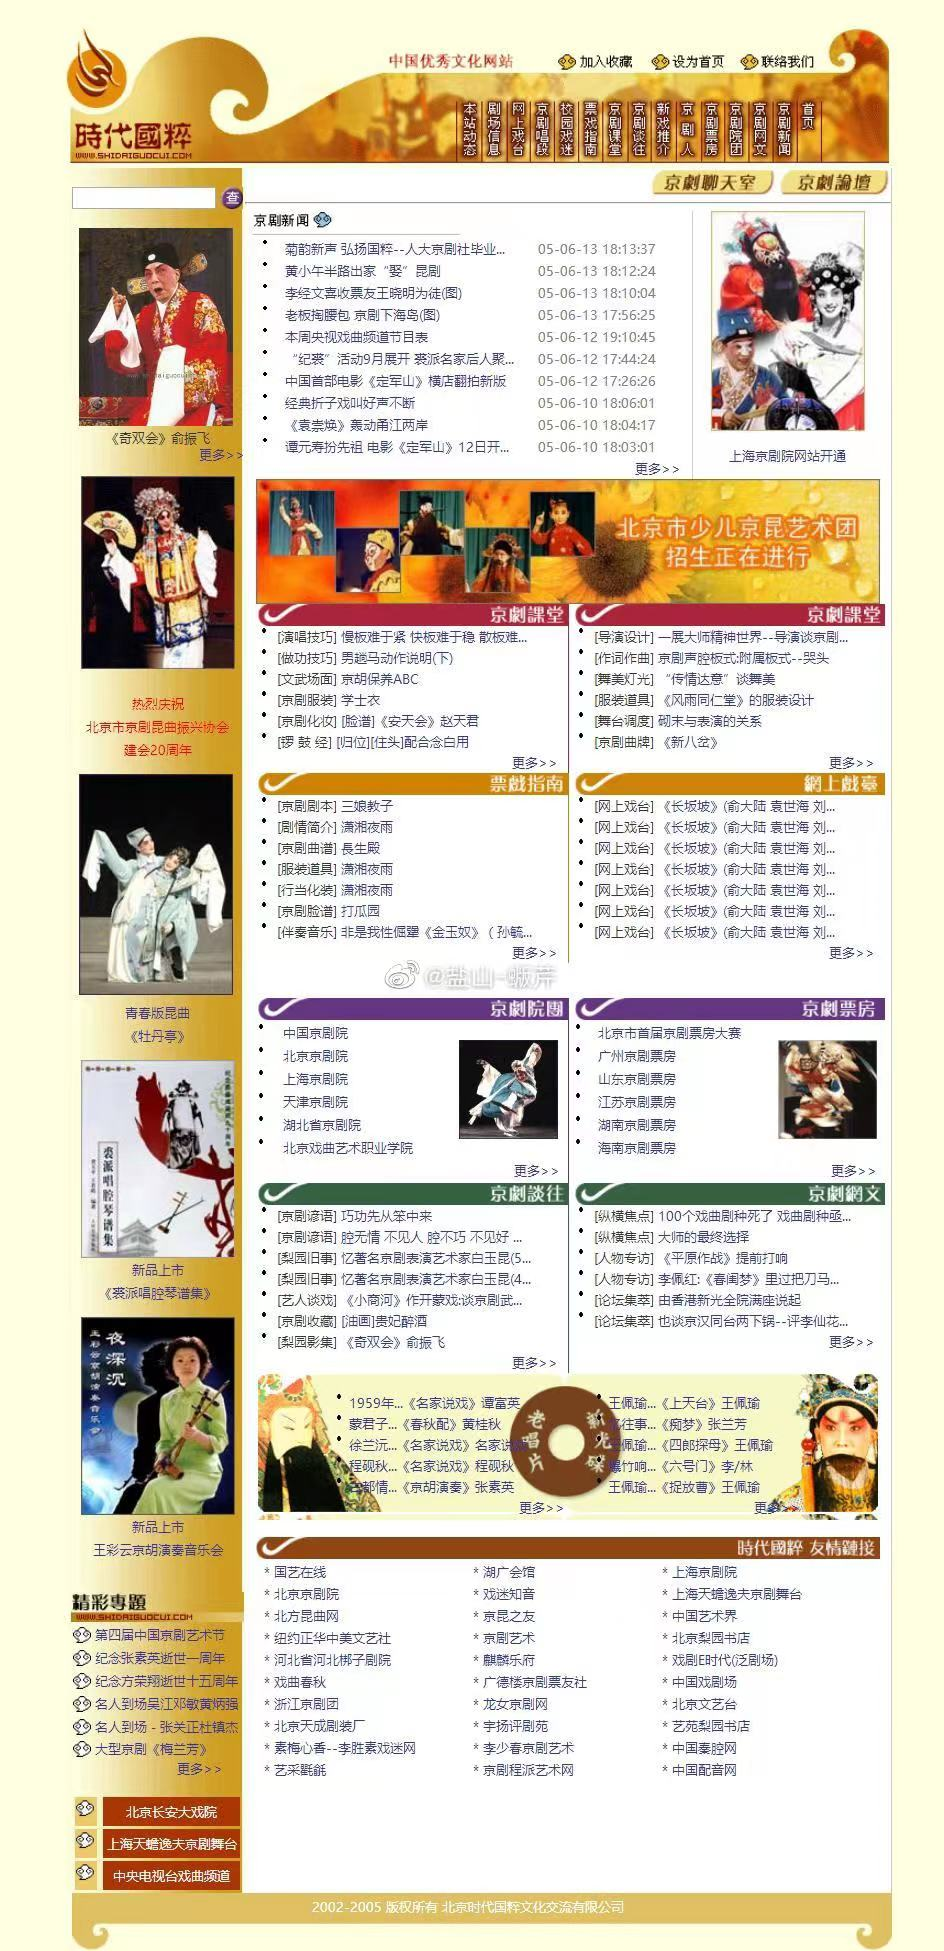
\includegraphics[height=0.8\textwidth,width=0.4\textwidth,clip]{Figures_Peking-Opera/PekOpe_Shidai.jpg}
\label{Shidai}
\end{figure}
}

\frame
{
	\frametitle{京剧艺术及其论坛}
\begin{figure}[h!]
\centering
\vspace{-0.2in}
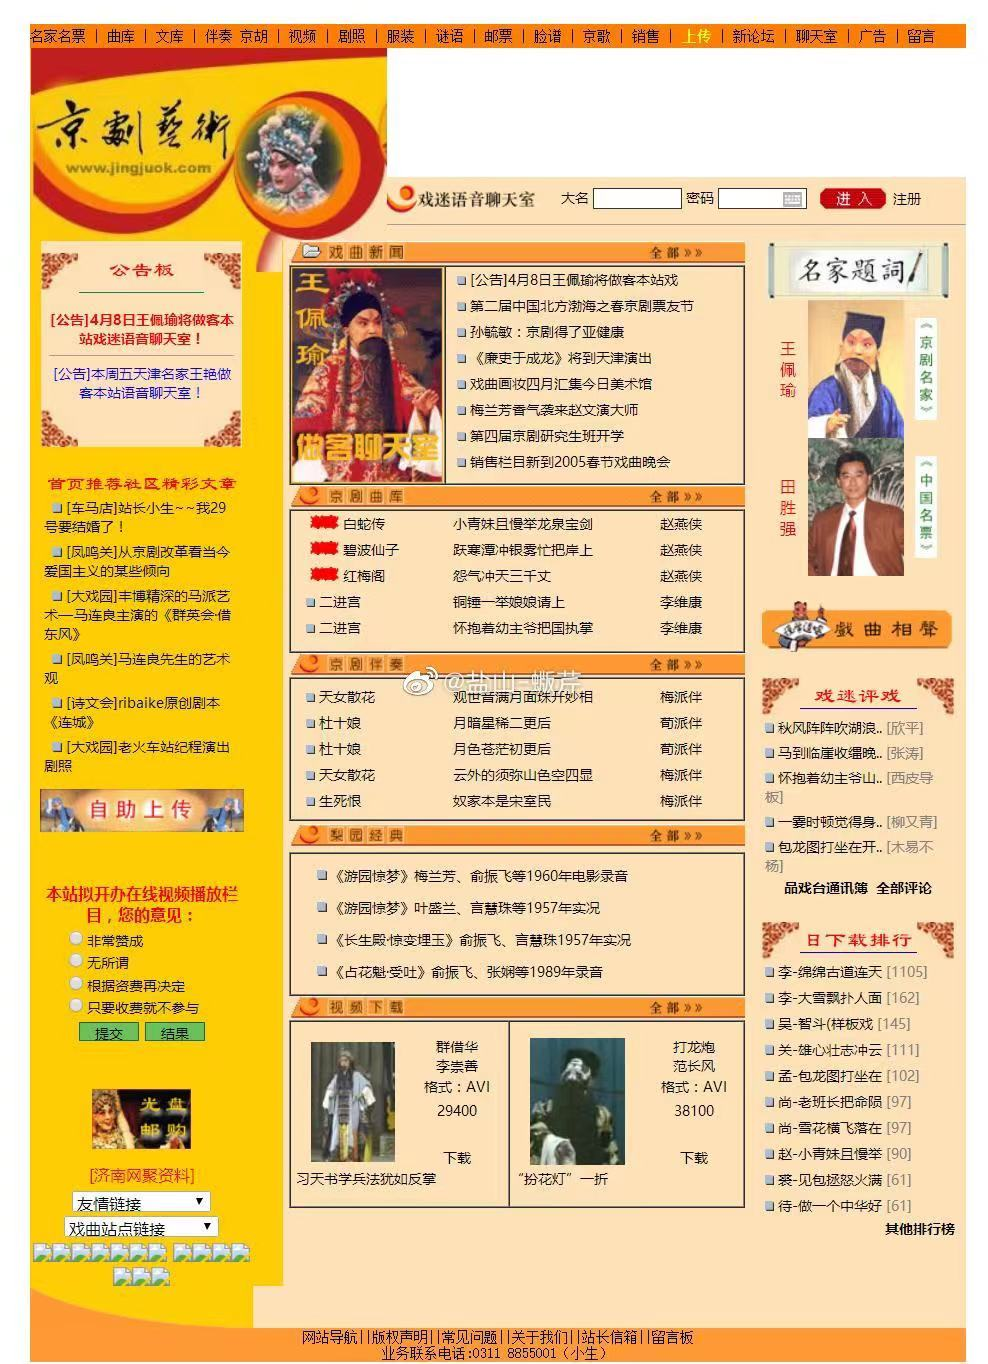
\includegraphics[height=0.8\textwidth,width=0.6\textwidth,clip]{Figures_Peking-Opera/PekOpe_Jingyi.jpg}
\label{Jingyi-1}
\end{figure}
}

\frame
{
	\frametitle{京剧艺术及其论坛}
\begin{figure}[h!]
\centering
\vspace{-0.3in}
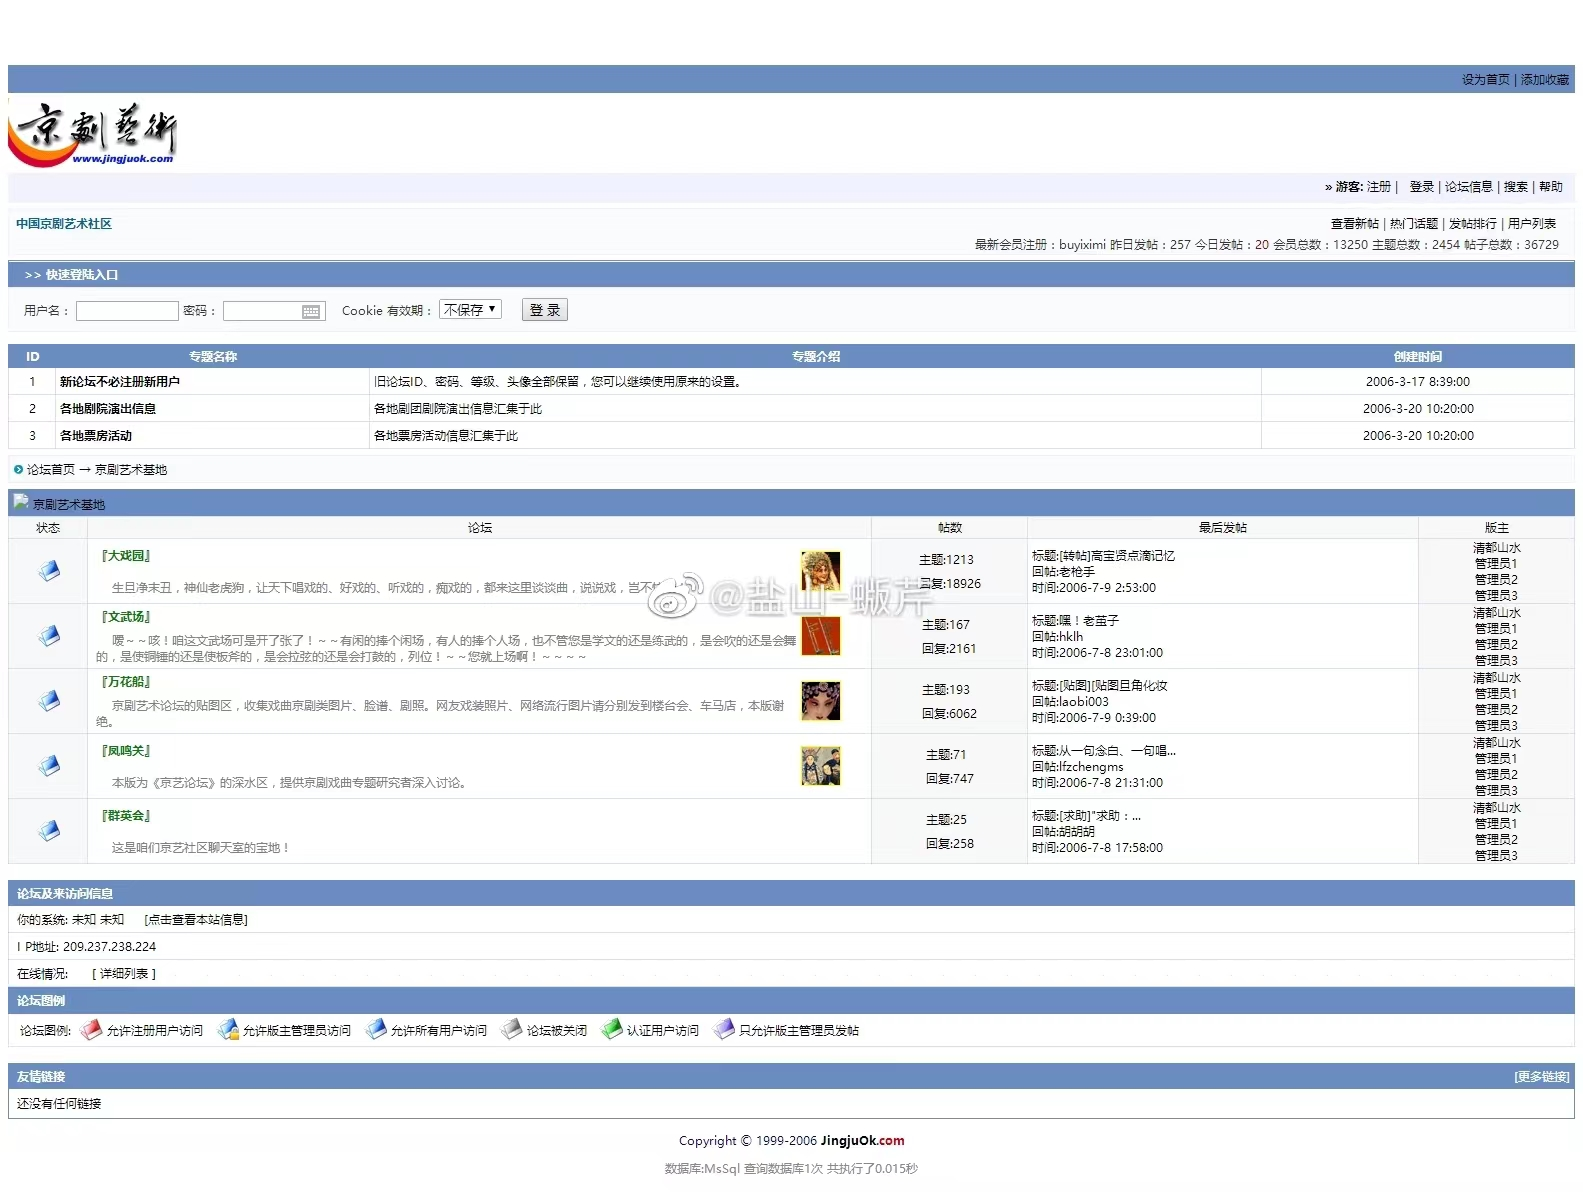
\includegraphics[height=0.75\textwidth,width=1.05\textwidth,clip]{Figures_Peking-Opera/PekOpe_Jingyilun.jpg}
\label{Jingyi-2}
\end{figure}
}

\frame
{
	\frametitle{听戏谈戏和梨园}
	梨园的名字源于网友“梨园\textrm{e}客”\\“听戏谈戏”最初的维护者是“豆腐”\\
	他们和“\textrm{xued}”和“皇兄”等共同开创了戏曲网站运营维护新模式
\begin{figure}[h!]
\centering
%\vspace{-0.05in}
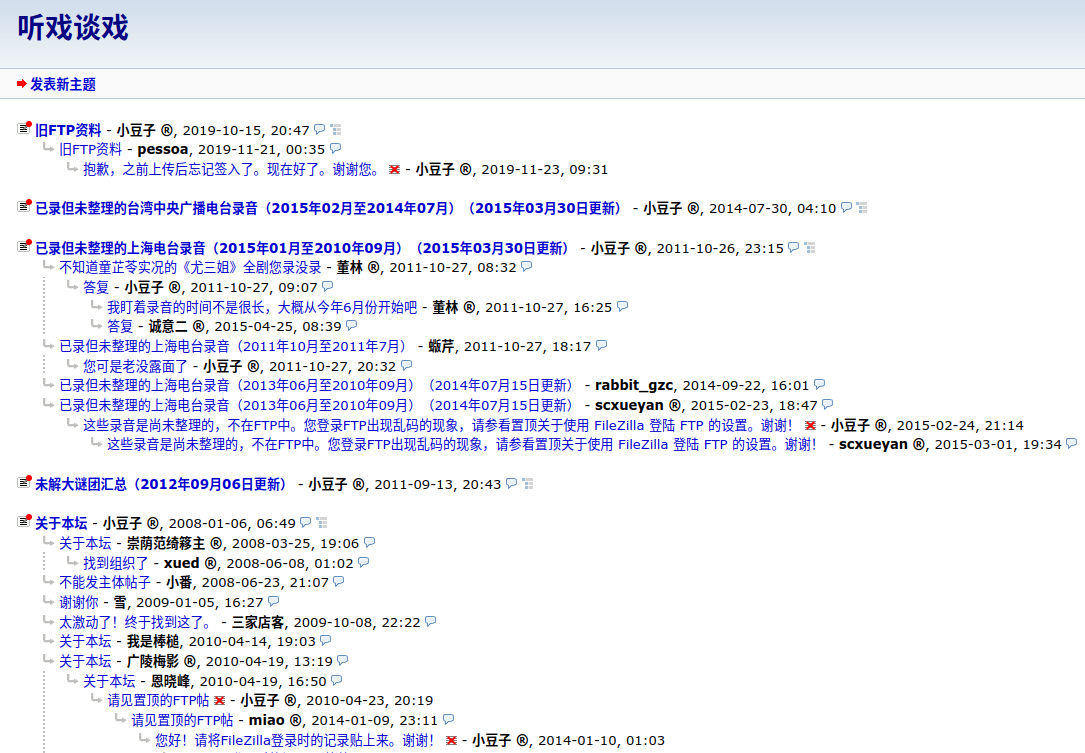
\includegraphics[height=0.55\textwidth,width=0.80\textwidth,clip]{Figures_Peking-Opera/PekOpe_Talk.png}
\label{Talk}
\end{figure}
}

\frame
{
	\frametitle{梨园、听戏谈戏和戏考、中国京剧老唱片}
	戏考是“小豆子”开发、管理和维护的京剧剧本数据库网站\\
	\textcolor{red}{互联网时代的梨园编年史记}
\begin{figure}[h!]
\centering
\vspace{-0.05in}
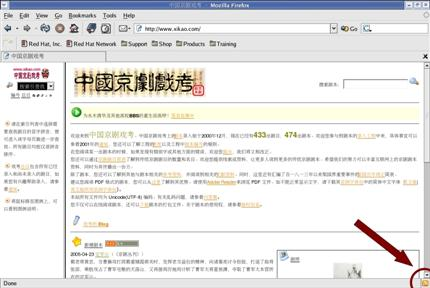
\includegraphics[height=0.60\textwidth,width=0.85\textwidth,clip]{Figures_Peking-Opera/PekOpe_Xikao.jpg}
\label{Xikao}
\end{figure}
}

\frame
{
	\frametitle{京剧方舟}
\begin{figure}[h!]
\centering
\vspace{-0.1in}
\hspace*{-0.15in}
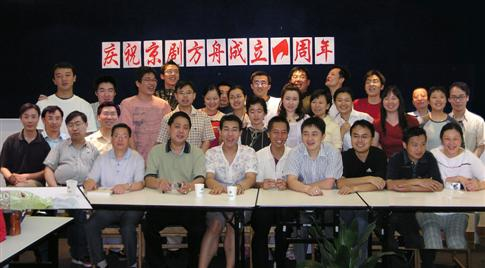
\includegraphics[height=0.60\textwidth,width=1.05\textwidth,clip]{Figures_Peking-Opera/PekOpe_Fangzhou.jpg}
\label{Fangzhou}
\end{figure}
}

\frame
{
	\frametitle{网络的双刃剑:~德云社\rm{vs}老车站剧社}
\begin{figure}[h!]
\centering
\vspace{-0.2in}
\hspace*{-0.15in}
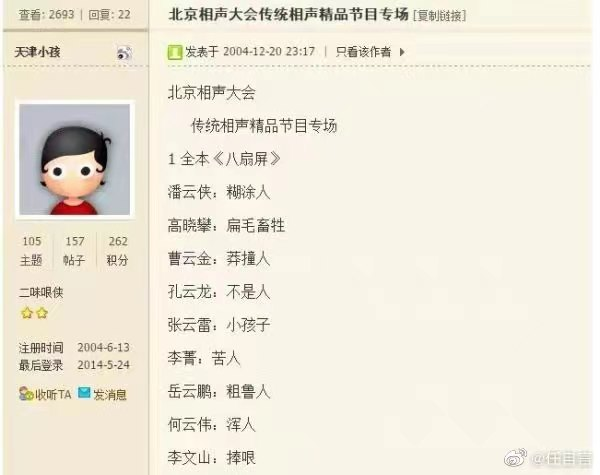
\includegraphics[height=0.35\textwidth,width=0.45\textwidth,clip]{Figures_Peking-Opera/PekOpe_Guo.jpg}
\vskip 1pt
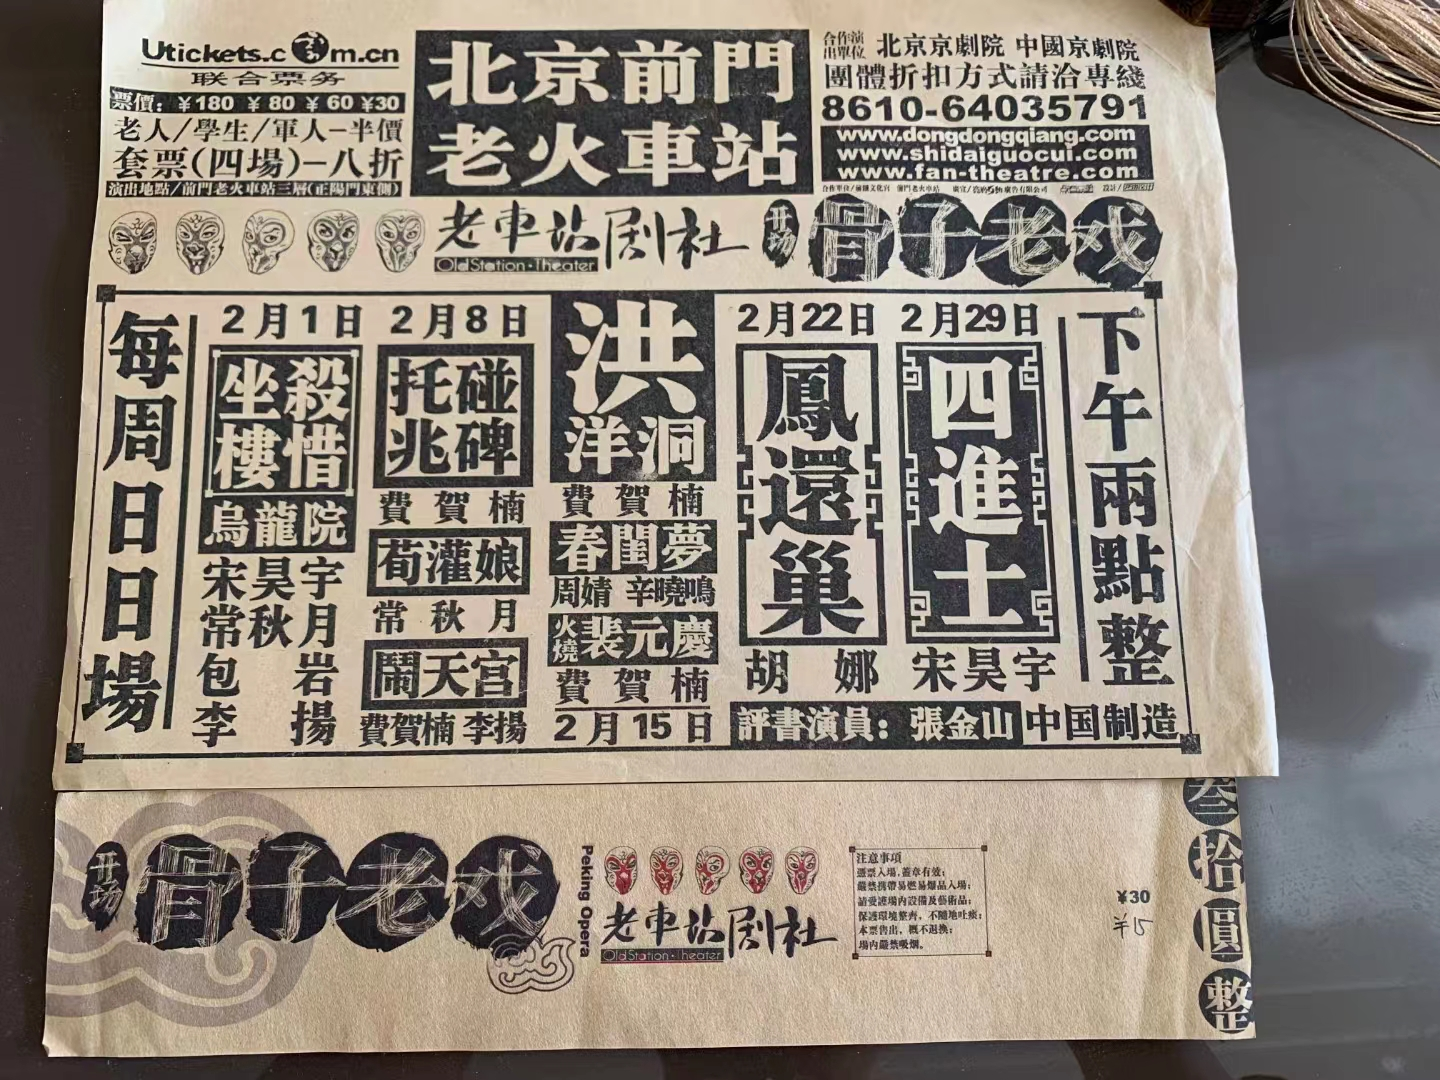
\includegraphics[height=0.40\textwidth,width=0.55\textwidth,clip]{Figures_Peking-Opera/PekOpe_Laochezhan-1.jpg}
%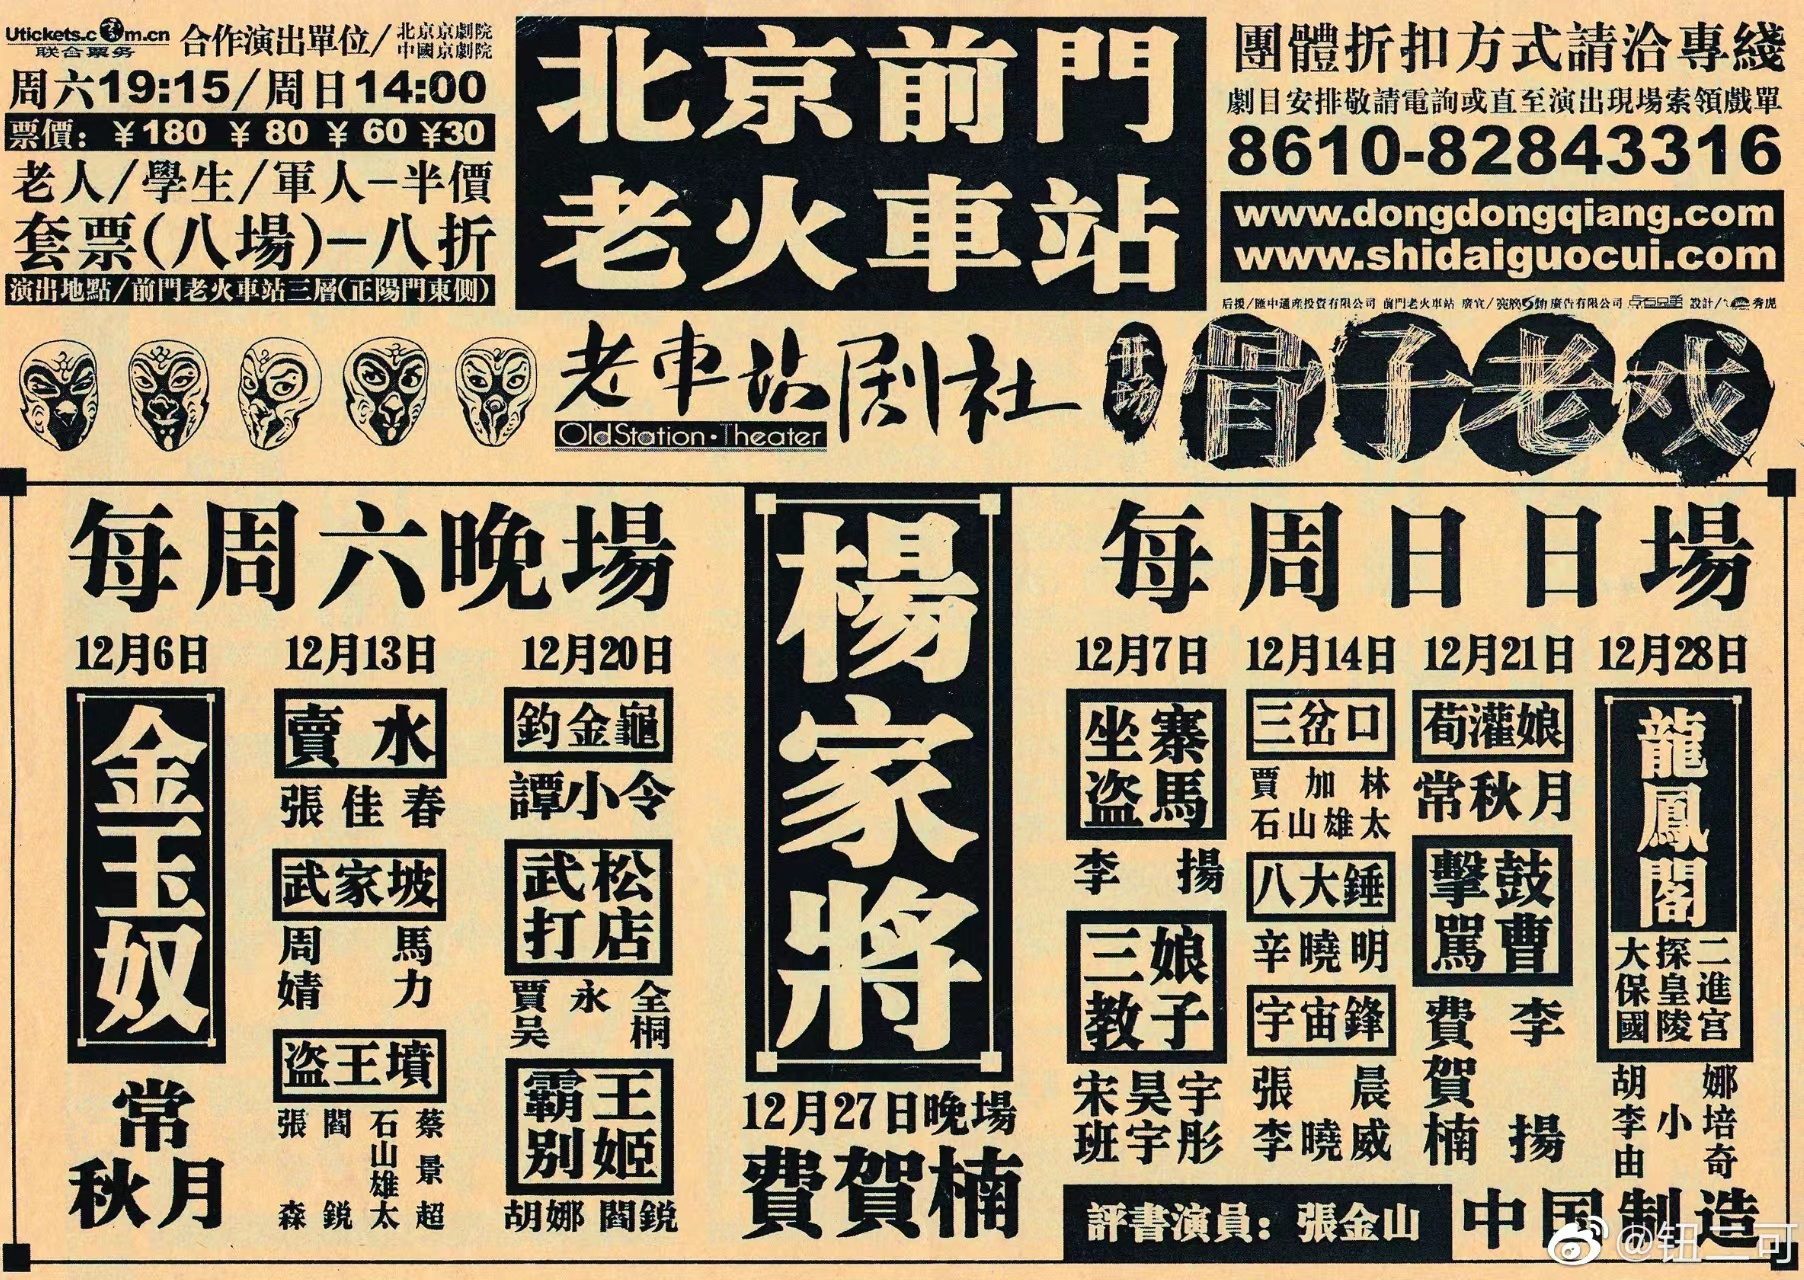
\includegraphics[height=0.40\textwidth,width=0.45\textwidth,clip]{Figures_Peking-Opera/PekOpe_Laochezhan-2.jpg}\\
\label{Guo_vs_Laochezhan}
\end{figure}
}

\section{传播:~资源与传承}
\subsection{网络:~推动京剧京剧资源的共享}
\frame
{
	\frametitle{北冥乘海生的\rm{FTP}}
	\textcolor{purple}{\textrm{FTP://166.111.67.33}~“相声网络传播的电和光,他是唯一的神话”}
\begin{figure}[h!]
\centering
\vspace{-0.05in}
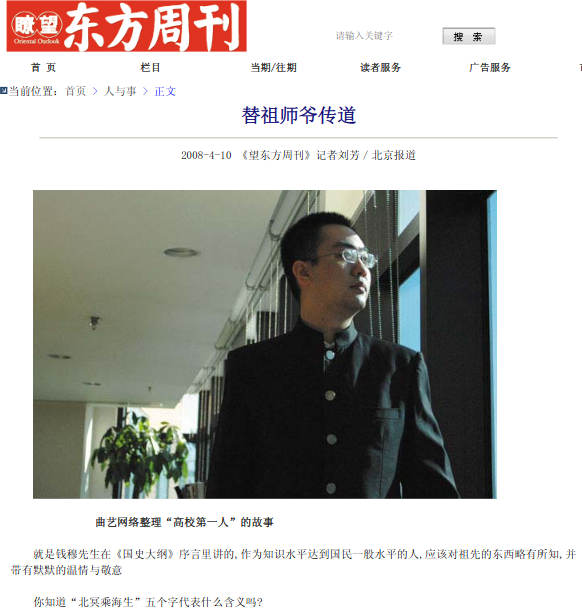
\includegraphics[height=0.60\textwidth,width=0.6\textwidth,clip]{Figures_Peking-Opera/PekOpe_Beiming.png}
\label{Beiming}
\end{figure}
}

\frame
{
	\frametitle{}
\begin{figure}[h!]
\centering
\vspace{-0.05in}
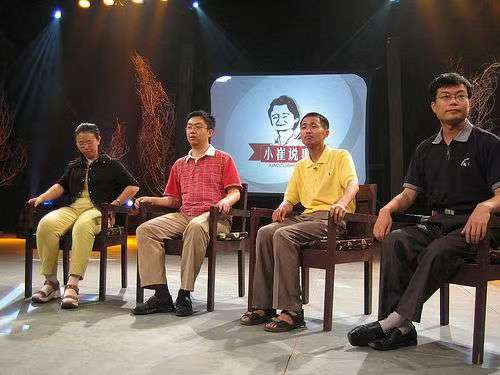
\includegraphics[height=0.60\textwidth,width=0.8\textwidth,clip]{Figures_Peking-Opera/PekOpe_Cui-1.jpg}
\label{Cui-1}
\end{figure}
}

\frame
{
	\frametitle{}
\begin{figure}[h!]
\centering
\vspace{-0.05in}
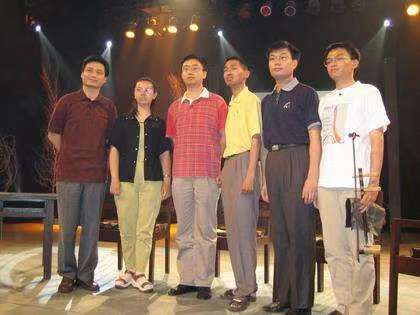
\includegraphics[height=0.60\textwidth,width=0.8\textwidth,clip]{Figures_Peking-Opera/PekOpe_Cui-2.jpg}
\label{Cui-2}
\end{figure}
\fontsize{6.0pt}{5.2pt}\selectfont{
	\url{https://www.bilibili.com/video/BV1eJ411H7d5?spm_id_from=333.337.search-card.all.click}}
}

\frame
{
	\frametitle{梨园和中国京剧老唱片}
	\textcolor{purple}{梨园:~永不关门的戏园子}
\begin{figure}[h!]
\centering
\vspace{-0.05in}
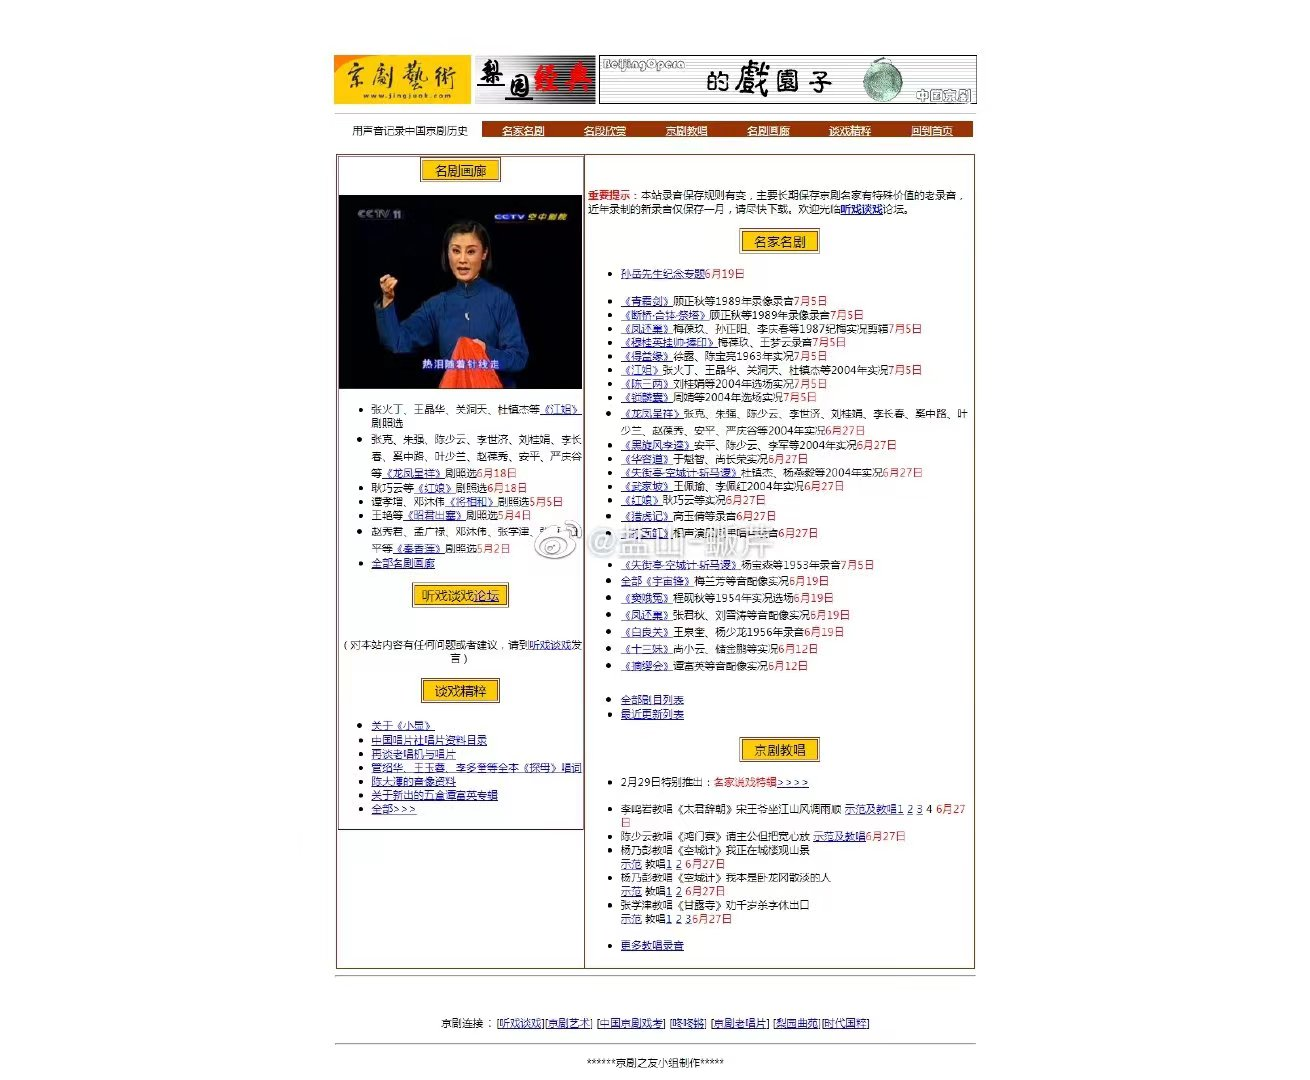
\includegraphics[height=0.65\textwidth,width=0.75\textwidth,clip]{Figures_Peking-Opera/PekOpe_Liyuan.jpg}
\label{Liyuan}
\end{figure}
}

\frame
{
	\frametitle{梨园和中国京剧老唱片}
	\textcolor{purple}{老唱片里的京剧历史}
\begin{figure}[h!]
\centering
\vspace{-0.05in}
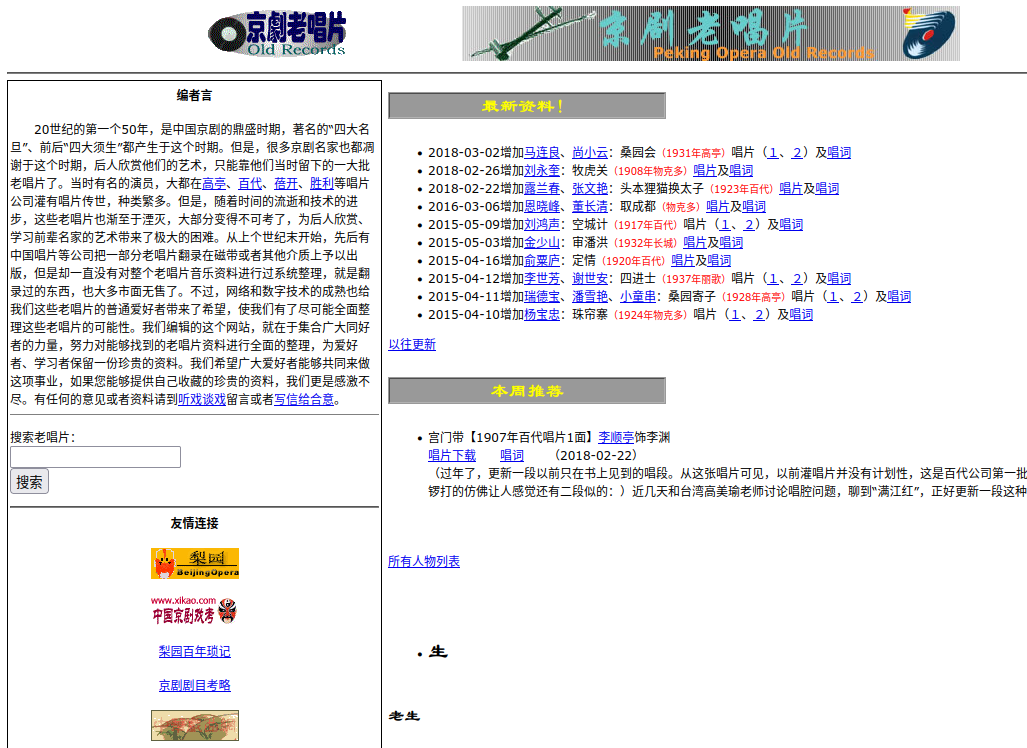
\includegraphics[height=0.65\textwidth,width=0.90\textwidth,clip]{Figures_Peking-Opera/PekOpe_Oldrec.png}
\label{Oldrecord}
\end{figure}
}

\frame
{
	\frametitle{网络:~传统京剧纪录的重要载体}
\begin{figure}[h!]
\centering
\vspace{-0.05in}
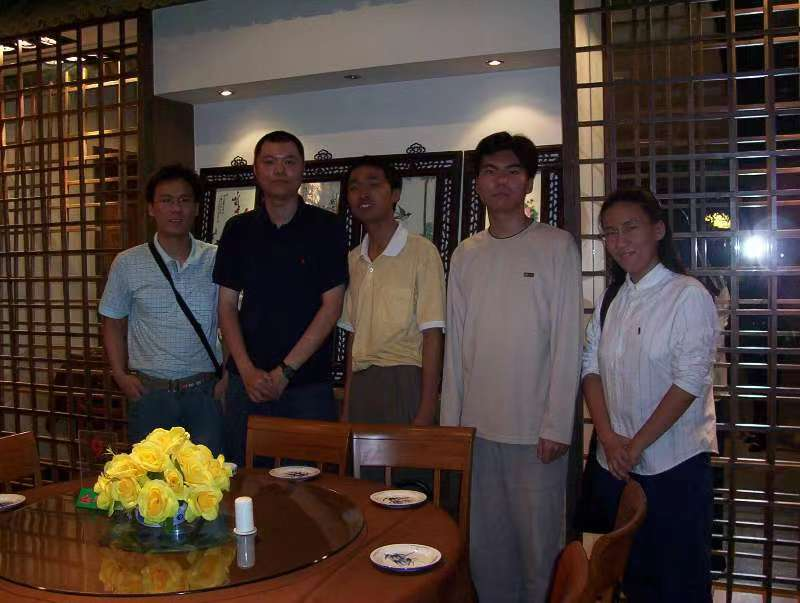
\includegraphics[height=0.65\textwidth,width=0.90\textwidth,clip]{Figures_Peking-Opera/PekOpe_Xiyou-1.jpg}
\label{Xiyou-1}
\end{figure}
}

\frame{
	\frametitle{}
	主要的传统京剧影音资料站点:~
	\begin{itemize}
		\item \textrm{FTP}类:
			\begin{itemize}
				\item 北冥乘海生的\textrm{FTP\\
					\url{FTP://166.111.67.33}~$\Rightarrow$~\url{FTP://162.105.89.74}}
				\item 京剧艺术的\textrm{FTP}~$\Rightarrow$~梨园的\textrm{FTP}
			\end{itemize}
		\item 各门户戏曲网站及其论坛:~京剧艺术论坛:~各类戏曲照片
		\item 玲珑戏曲网论坛:~戏曲、曲艺录音(主要由“凤点头”、“西城老军”等网友贡献),促进两岸网友戏曲资料的互动
		\item 戏曲流传的戏曲资料日趋丰富:~视频(土豆网)、全剧录音(梨园)、剧本资源(戏考)、京剧老唱片
	\end{itemize}
	\underline{\textrm{FTP}模式}便于影音资源集中和分享,但网络链接不稳定\\
	\underline{论坛模式}更主要的功能是交流,分享戏曲图片、影音资源分散\\
	后期,\underline{梨园\textrm{FTP}}是两岸网友戏曲资料分享的主要载体
}

\frame
{
	\frametitle{网络:~海峡两岸传统京剧交流的平台}
	\textrm{2004}年起,两岸网友通过分享录音的方式交流了一大批珍贵录音
\begin{figure}[h!]
\centering
\vspace{-0.05in}
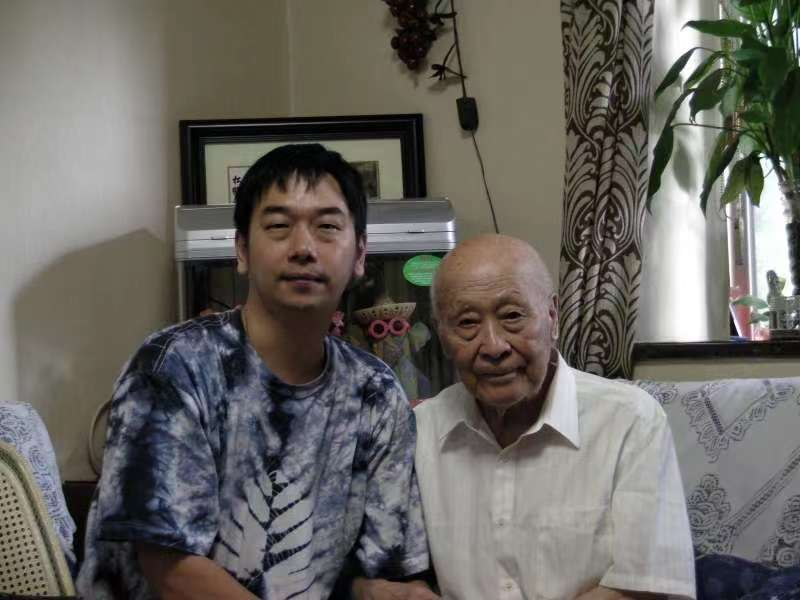
\includegraphics[height=0.6\textwidth,width=0.85\textwidth,clip]{Figures_Peking-Opera/PekOpe_Li-1.jpg}
\label{Li-1}
\end{figure}
}

\frame
{
	\frametitle{}
\begin{figure}[h!]
\centering
\vspace{-0.05in}
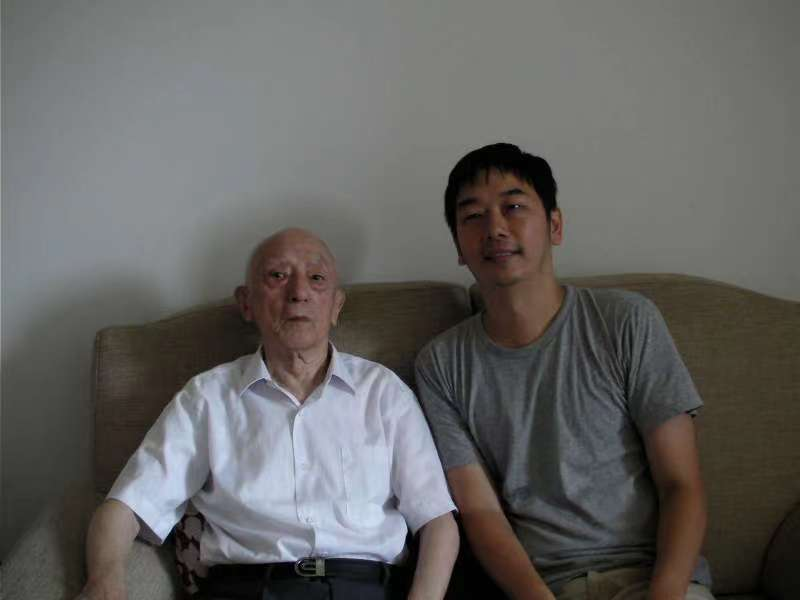
\includegraphics[height=0.6\textwidth,width=0.85\textwidth,clip]{Figures_Peking-Opera/PekOpe_Li-2.jpg}
\label{Li-2}
\end{figure}
}

\frame
{
	\frametitle{}
\begin{figure}[h!]
\centering
\vspace{-0.05in}
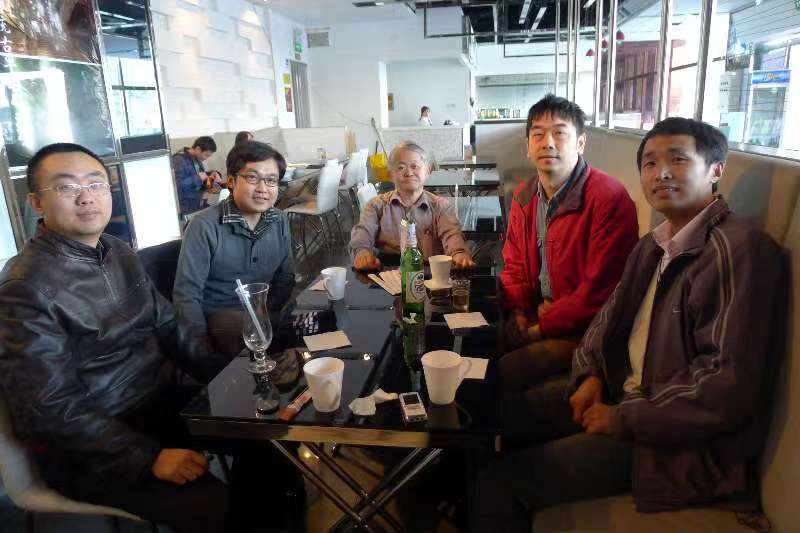
\includegraphics[height=0.6\textwidth,width=0.85\textwidth,clip]{Figures_Peking-Opera/PekOpe_Xiyou-2.jpg}
\label{Xiyou-2}
\end{figure}
}

\frame
{
	\frametitle{网络:~继续传统京剧精神的民间相传}
	\begin{itemize}
   		\setlength{\itemsep}{15pt}
		\item 《粉墨春秋》
		\item 《百年京剧》
		\item 《风雨样板戏》
	\end{itemize}
	\textcolor{red}{个人理想}:\\
\textcolor{blue}{已数字化的戏曲资源实现完全开源分享并“去中心化”,越珍贵的资料越应该人手一份,保证这些材料不遗失的唯一最可靠途径}
}

\subsection{网络:~推动京剧研究思想的流传~(以“九三三老”为例)}
\frame
{
	\frametitle{朱家溍先生:~古典审美的修养}
\begin{figure}[h!]
\centering
\vspace{-0.1in}
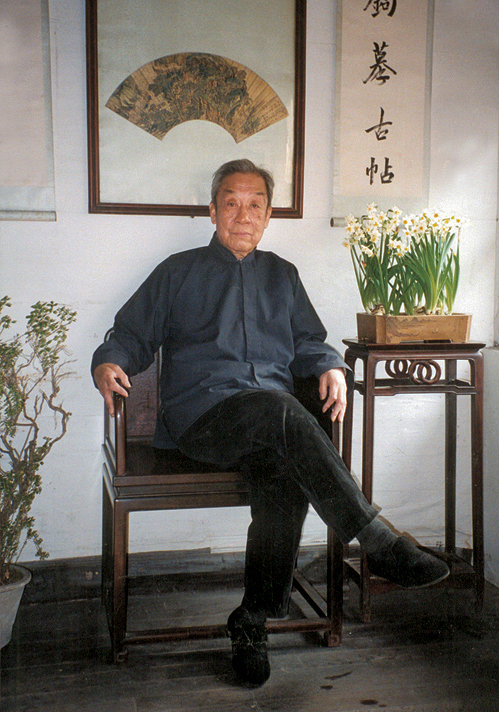
\includegraphics[height=0.64\textwidth,width=0.46\textwidth,viewport=0 0 500 720,clip]{Figures_Peking-Opera/Zhu_Jiajin.jpg}
\hskip 5pt
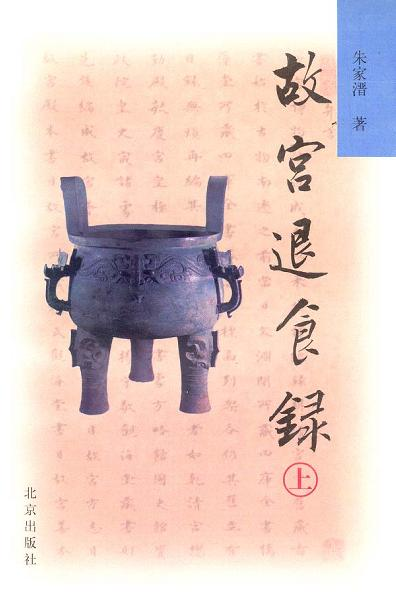
\includegraphics[height=0.64\textwidth,width=0.46\textwidth,viewport=0 0 450 610,clip]{Figures_Peking-Opera/Zhu_Tuishilu.jpg}
%\caption{朱家溍先生}
\label{Zhu_Jiajin}
\end{figure}
}

\frame
{
	\frametitle{}
\begin{figure}[h!]
\centering
\vspace{-0.15in}
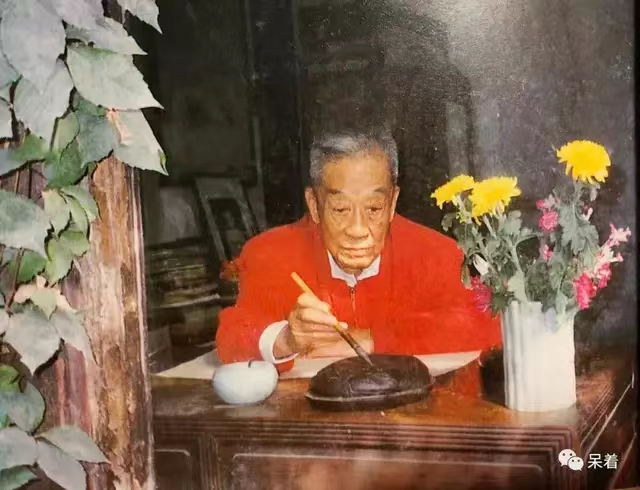
\includegraphics[height=0.65\textwidth,width=0.80\textwidth,clip]{Figures_Peking-Opera/PekOpe_Zhu.jpg}
\label{Zhu_Jiajin-2}
\end{figure}
}

\frame
{
	\frametitle{刘曾复先生:~科学整合的思想}
\begin{figure}[h!]
\centering
\vspace{-0.2in}
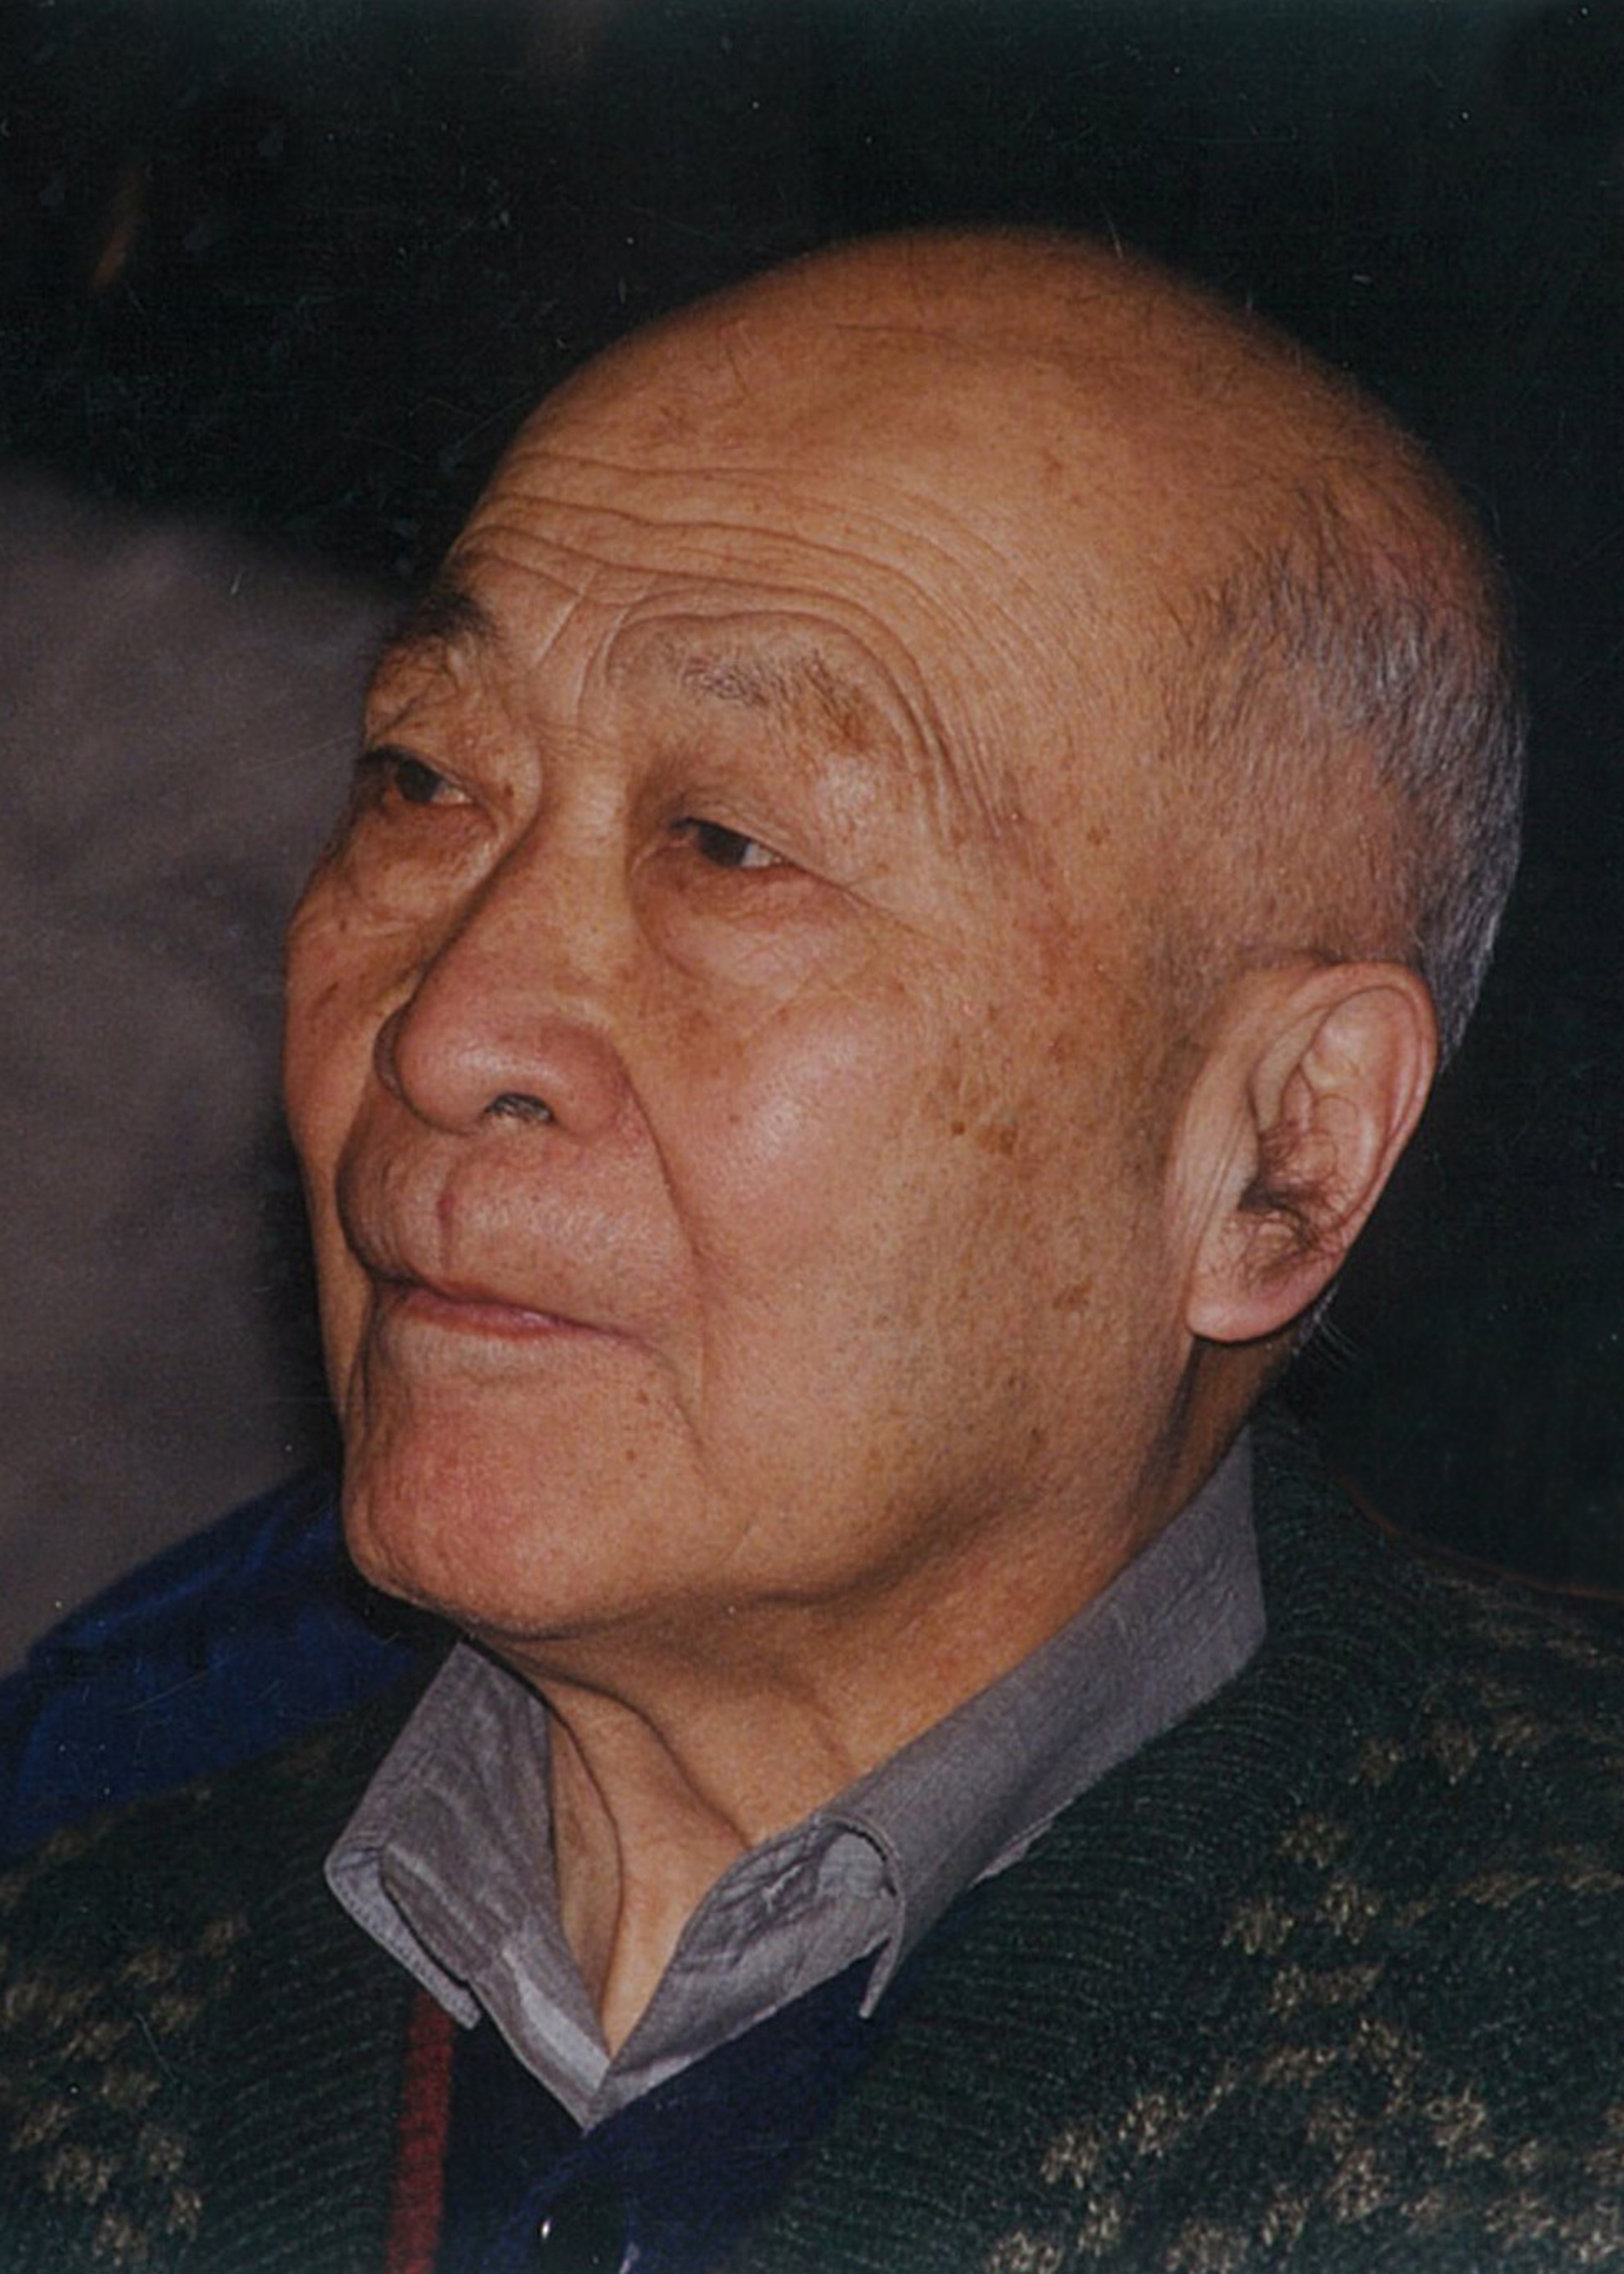
\includegraphics[height=0.64\textwidth,width=0.46\textwidth,viewport=0 0 360 520,clip]{Figures_Peking-Opera/Liu_Zengfu.jpg}
\hskip 5pt
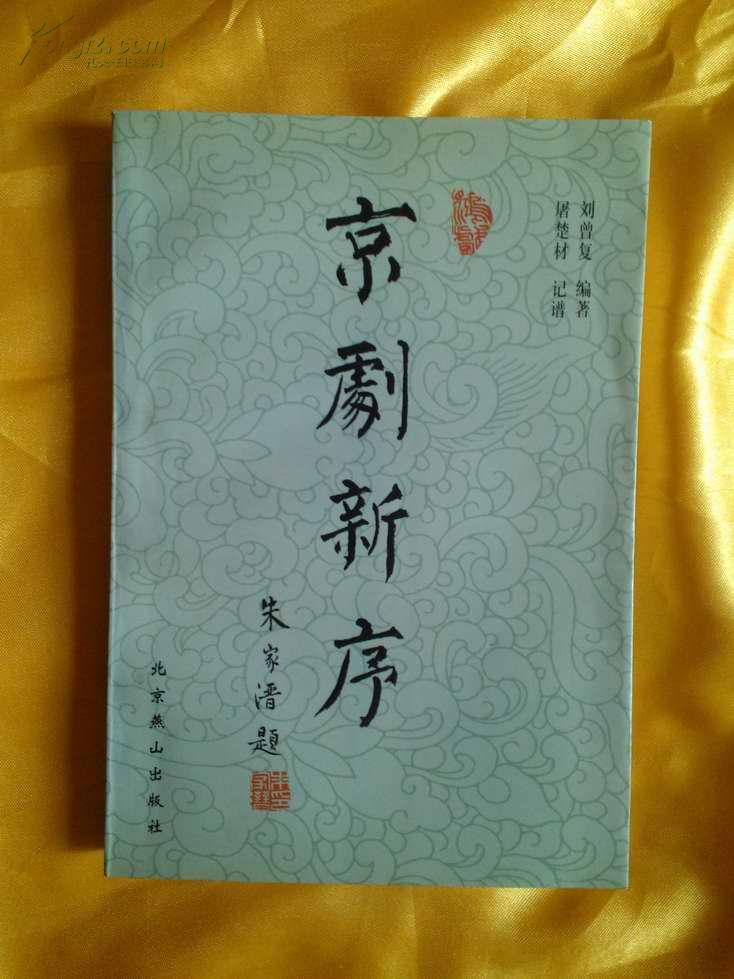
\includegraphics[height=0.62\textwidth,width=0.45\textwidth,viewport=100 85 660 875,clip]{Figures_Peking-Opera/Liu_Xinxu.jpg}
%\caption{刘曾复先生}
\label{Liu_Zengfu}
\end{figure}
}

\frame
{
	\frametitle{}
\begin{figure}[h!]
\centering
\vspace{-0.15in}
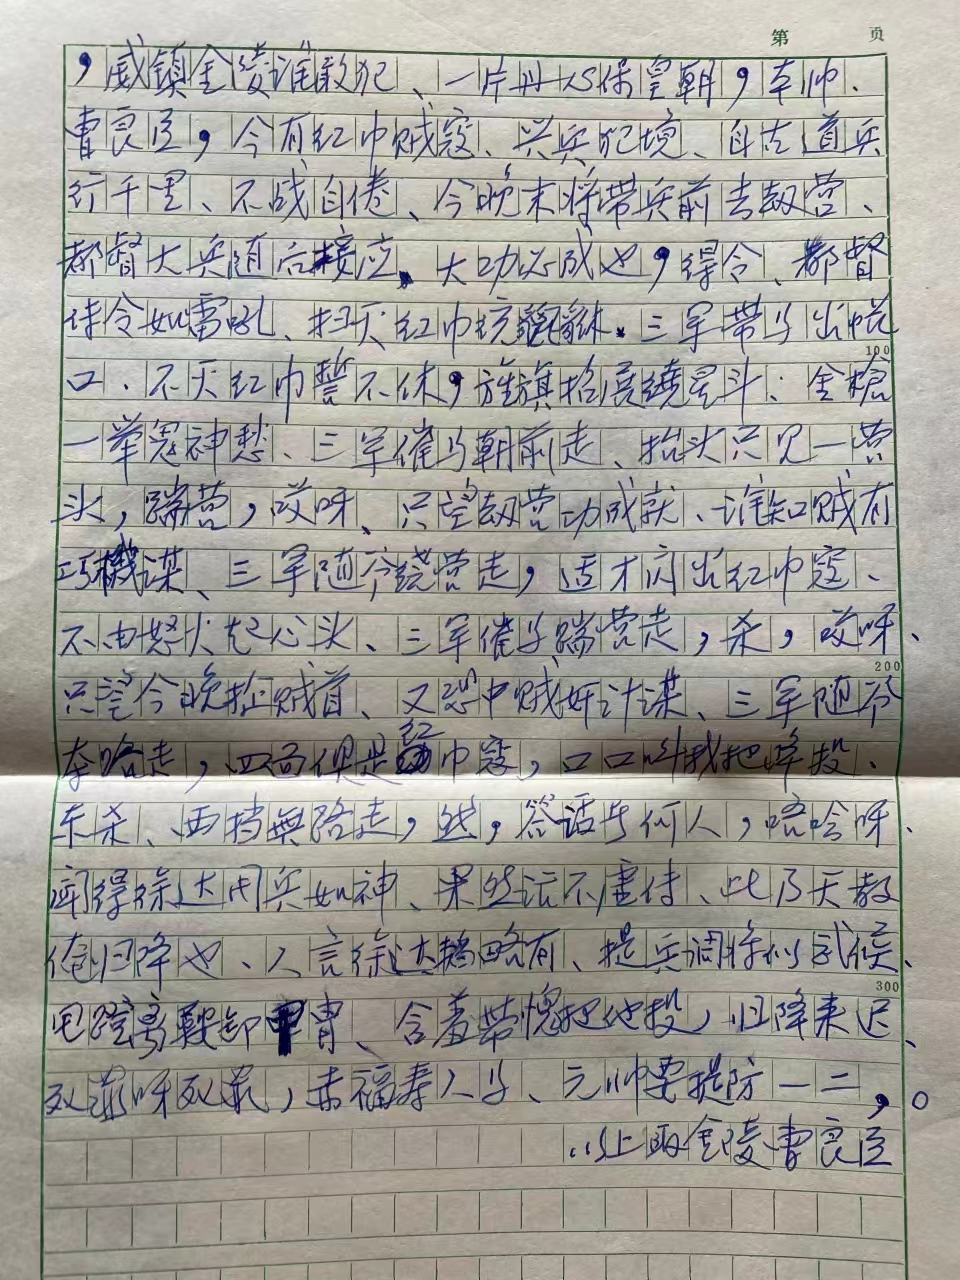
\includegraphics[height=0.72\textwidth,width=0.50\textwidth,clip]{Figures_Peking-Opera/PekOpe_Liu-1.jpg}
\hskip 1pt
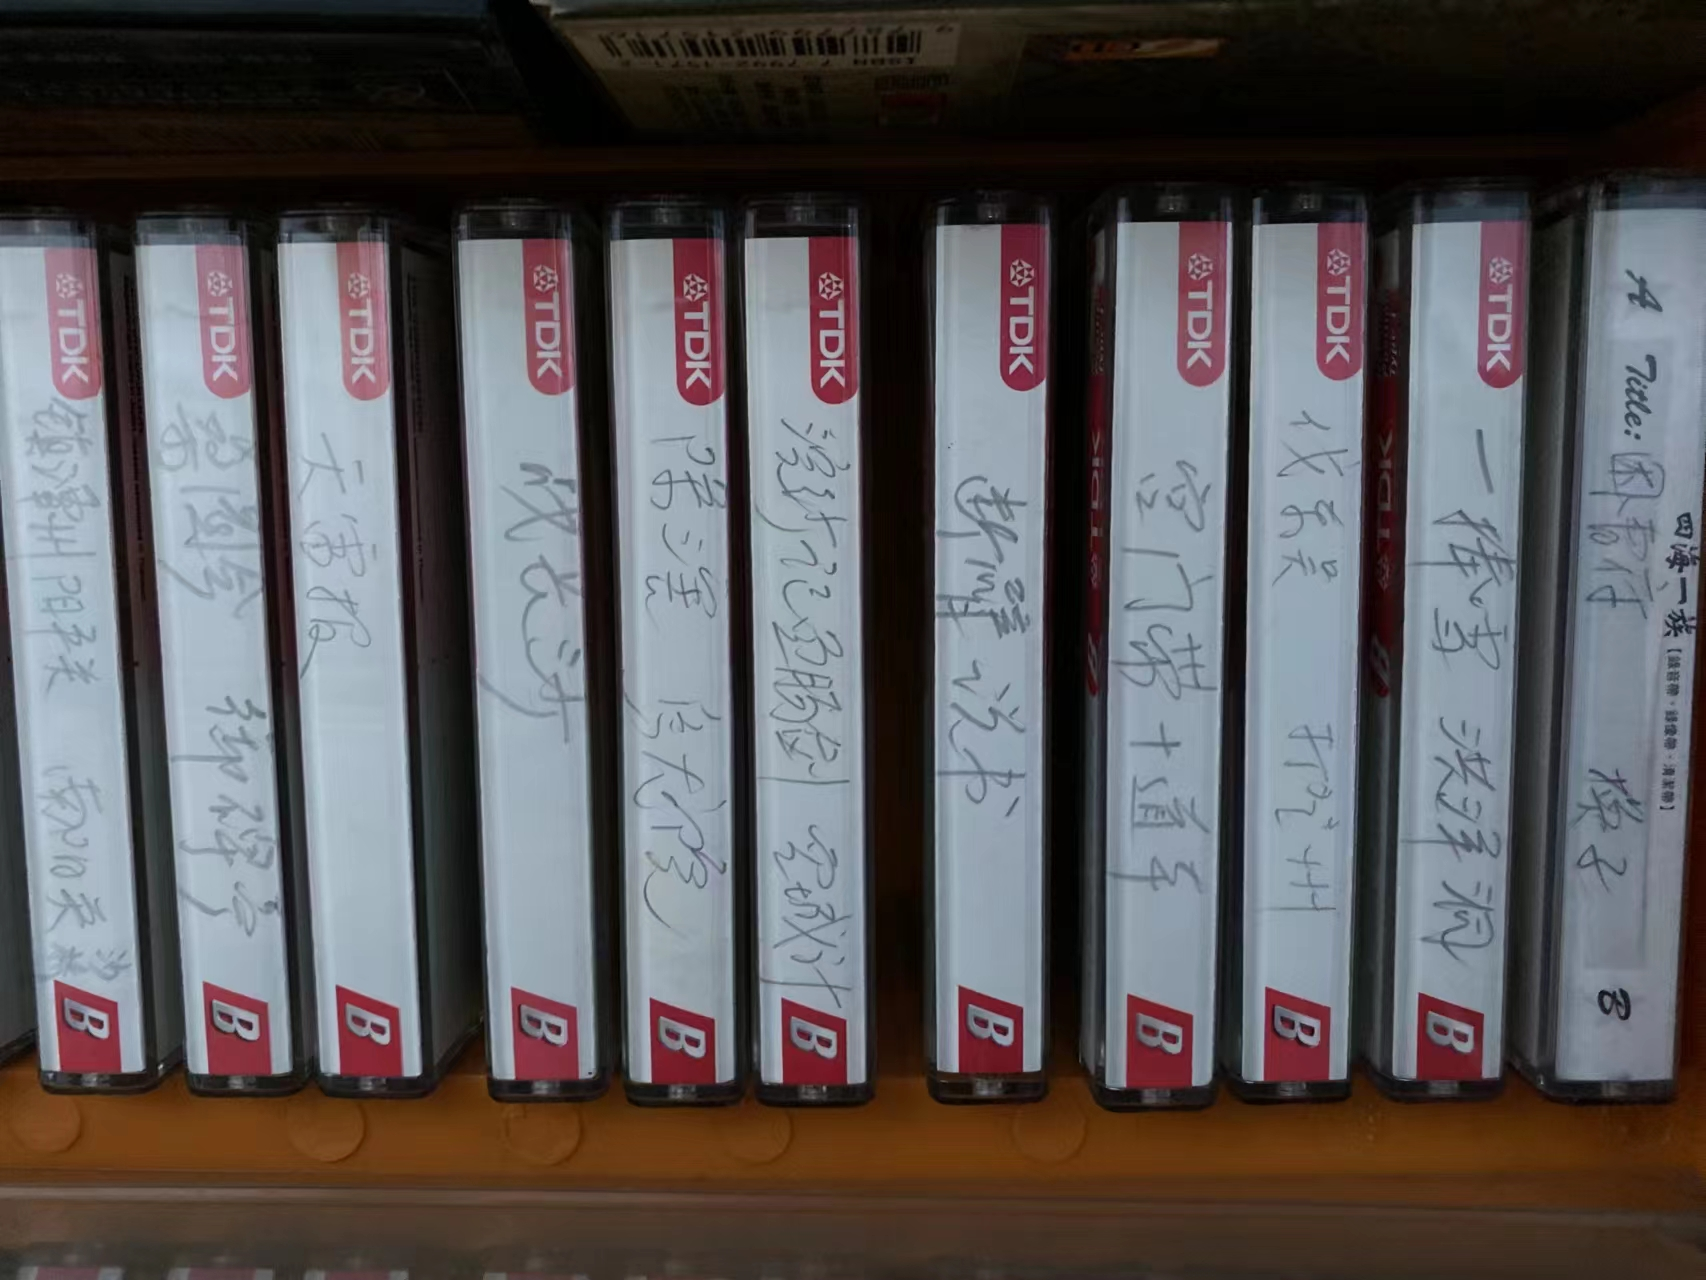
\includegraphics[height=0.35\textwidth,width=0.45\textwidth,clip]{Figures_Peking-Opera/PekOpe_Liu-2.jpg}
\label{Liu_Zengfu-2}
\end{figure}
}

\frame
{
	\frametitle{}
\begin{figure}[h!]
\centering
\vspace{-0.15in}
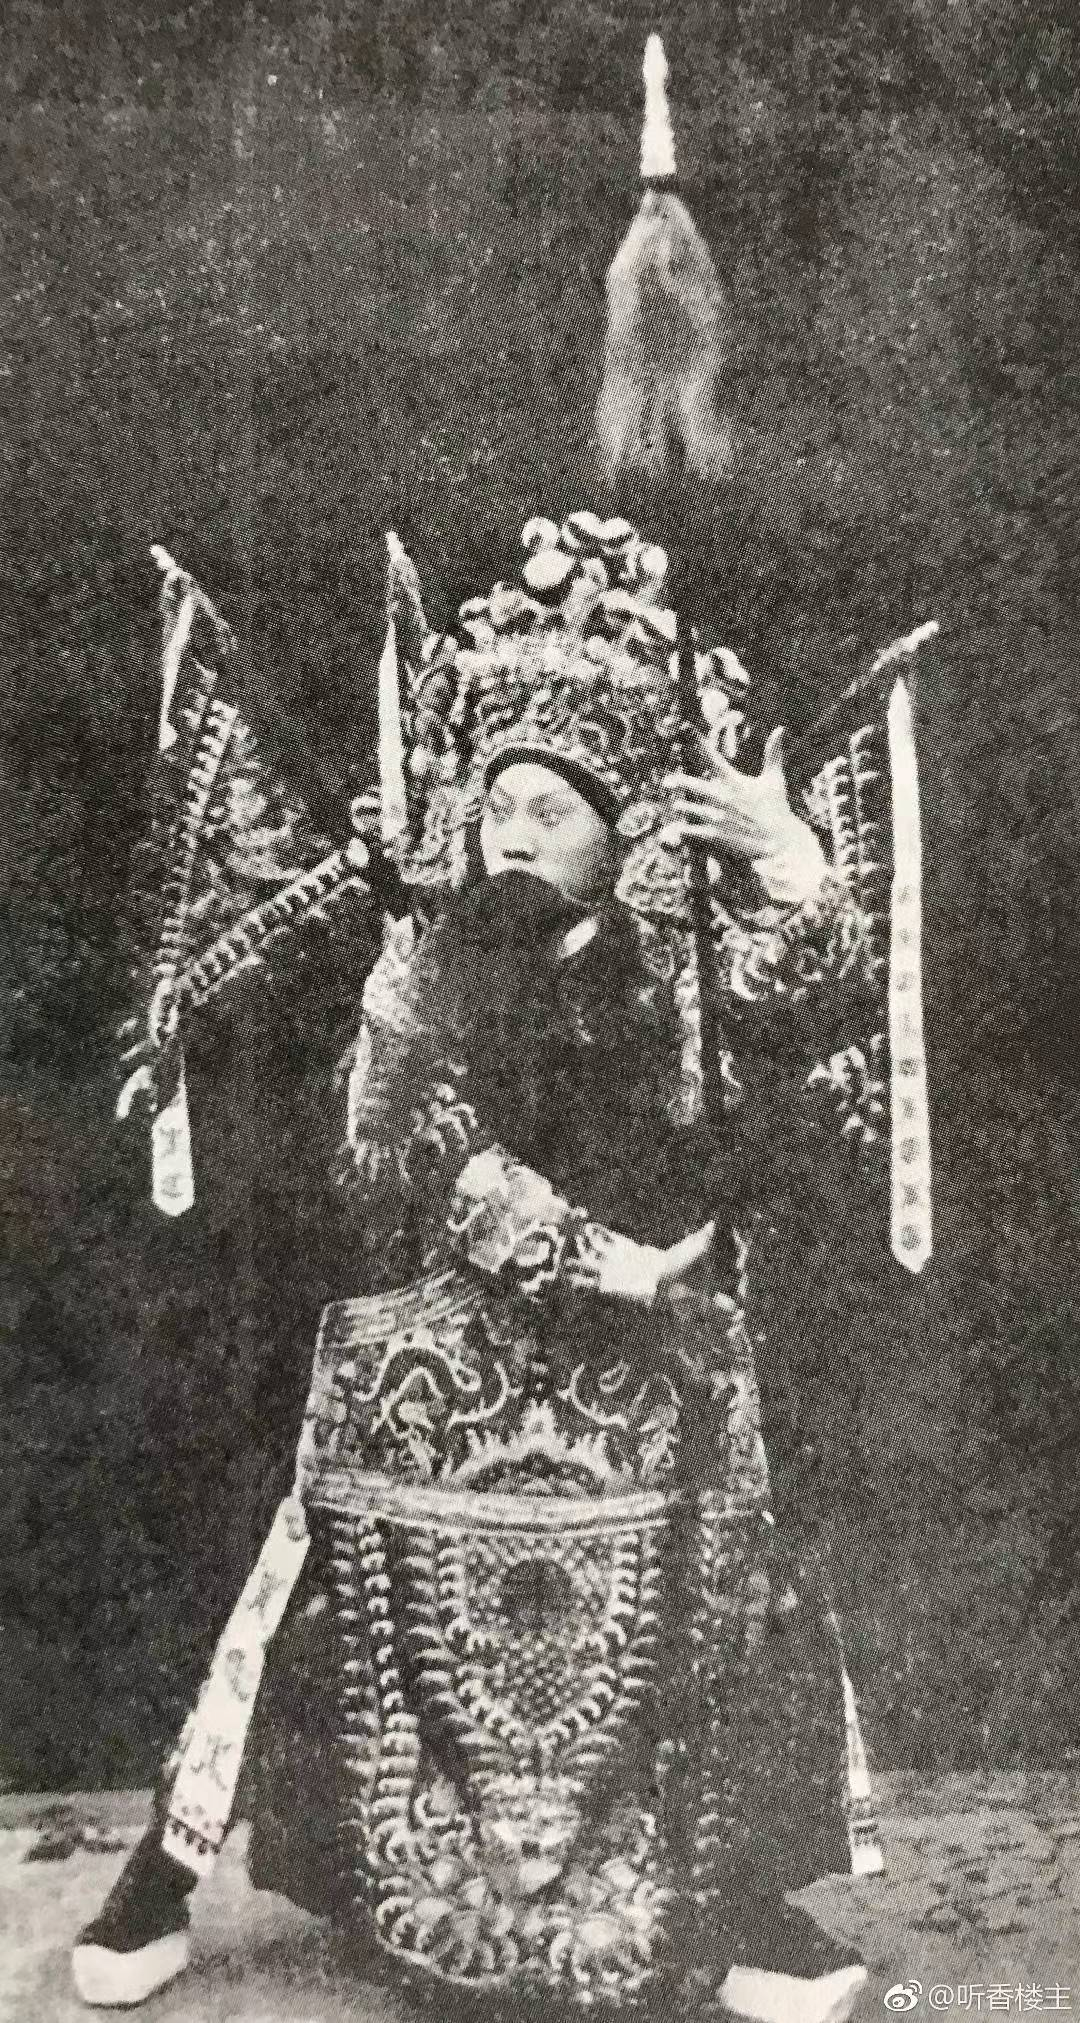
\includegraphics[height=0.64\textwidth,width=0.32\textwidth,clip]{Figures_Peking-Opera/PekOpe_Liu-3.jpg}
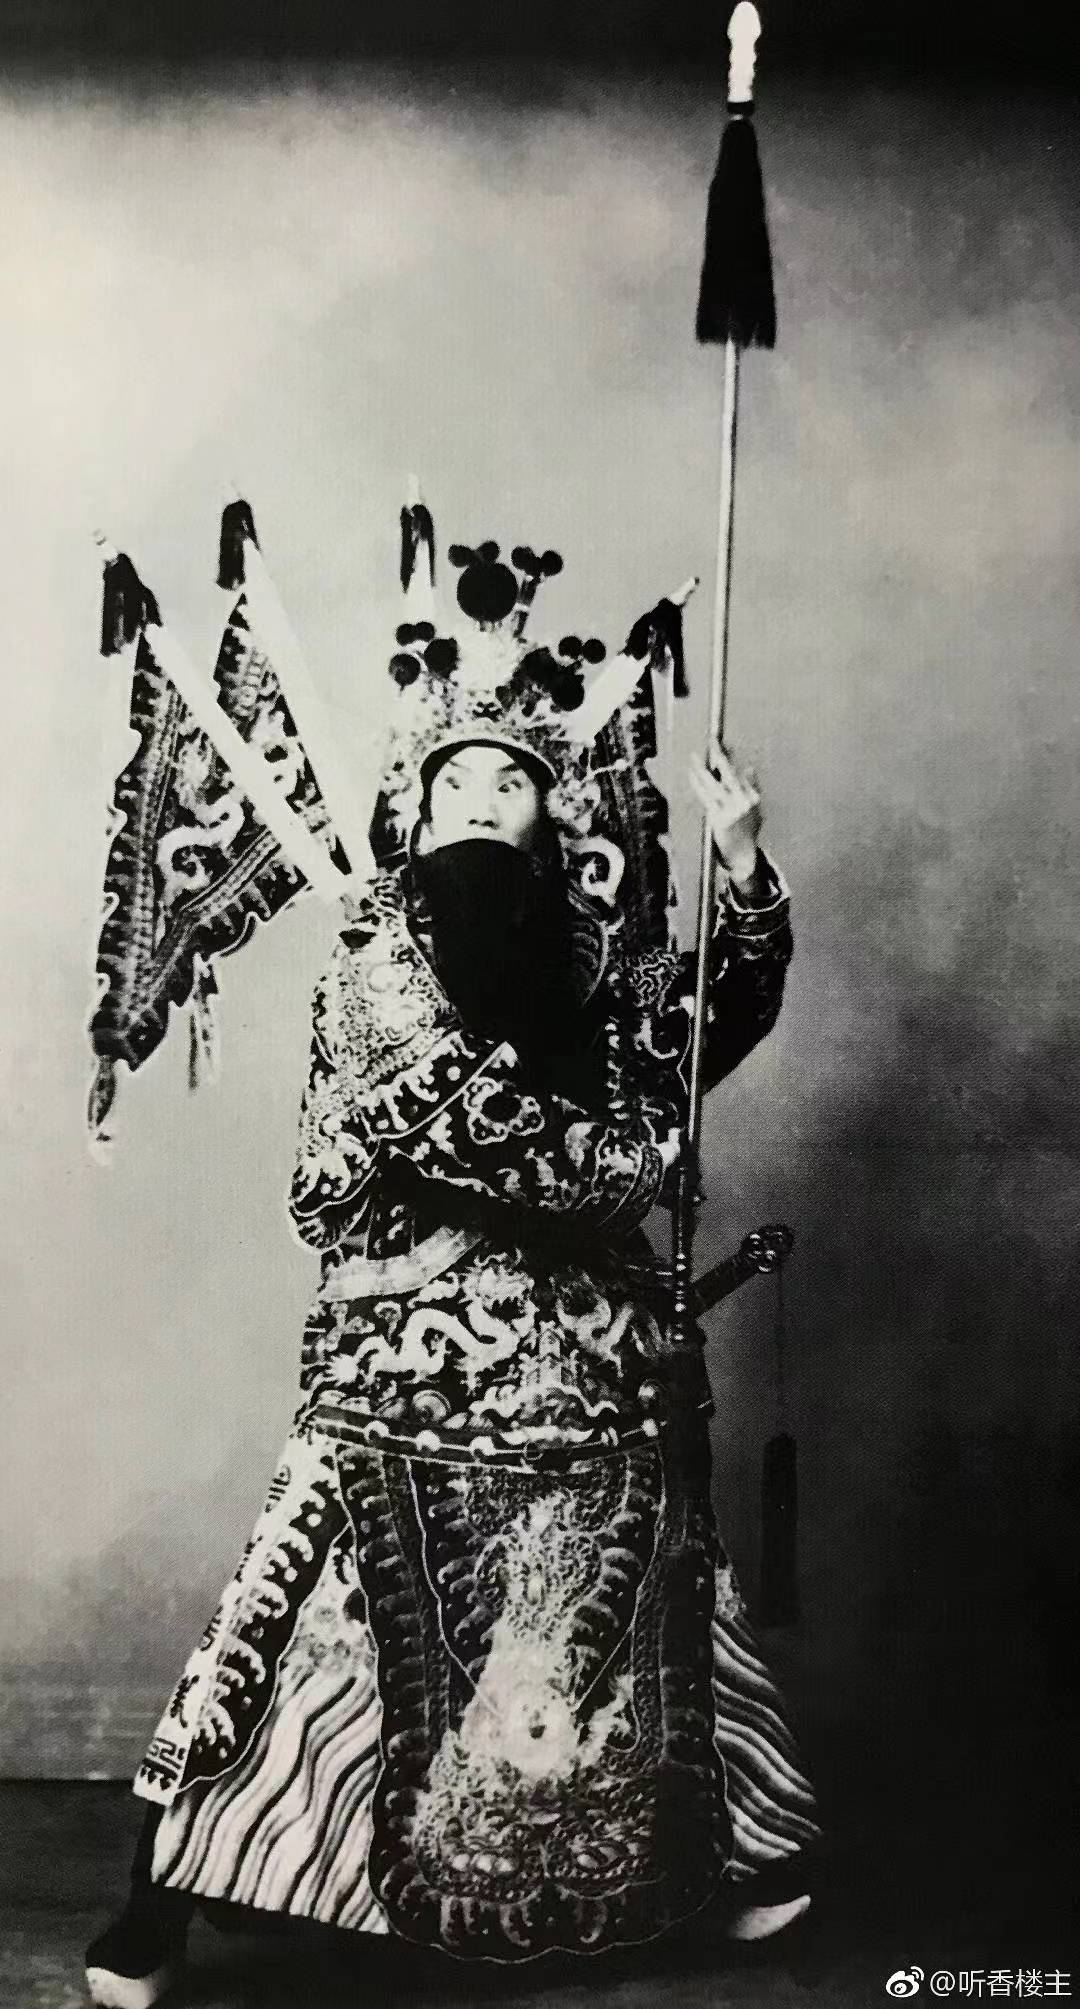
\includegraphics[height=0.64\textwidth,width=0.32\textwidth,clip]{Figures_Peking-Opera/PekOpe_Liu-4.jpg}
\includegraphics[height=0.60\textwidth,width=0.33\textwidth,clip]{Figures_Peking-Opera/PekOpe_Liu-5.jpg}
\label{Liu_Zengfu-3}
\end{figure}
}

\frame
{
	\frametitle{吴小如先生:~严谨认真的态度}
\begin{figure}[h!]
\centering
\vspace{-0.2in}
\includegraphics[height=0.64\textwidth,width=0.46\textwidth,viewport=0 0 360 520,clip]{Figures_Peking-Opera/Wu_Xiaoru.jpg}
\hskip 5pt
\includegraphics[height=0.64\textwidth,width=0.46\textwidth,viewport=39 5 200 235,clip]{Figures_Peking-Opera/Wu_Wenlu.jpg}
%\caption{吴小如先生}
\label{Wu_Xiaoru}
\end{figure}
}

\frame
{
	\frametitle{}
\begin{figure}[h!]
\centering
\vspace{-0.15in}
\includegraphics[height=0.45\textwidth,width=0.65\textwidth,clip]{Figures_Peking-Opera/PekOpe_Wu-1.jpg}
\vskip -25pt
\includegraphics[height=0.45\textwidth,width=0.65\textwidth,clip]{Figures_Peking-Opera/PekOpe_Wu-2.jpg}
\label{Wu_xiaoru-2}
\end{figure}
}

\frame
{
	\frametitle{}
\begin{figure}[h!]
\centering
\vspace{-0.15in}
\includegraphics[height=0.65\textwidth,width=1.00\textwidth,clip]{Figures_Peking-Opera/PekOpe_Wu-3.jpg}
\label{Wu_xiaoru-3}
\end{figure}
}

\frame
{
	\frametitle{}
\begin{figure}[h!]
\centering
\vspace{-0.15in}
%\includegraphics[height=0.45\textwidth,width=0.65\textwidth,clip]{Figures_Peking-Opera/PekOpe_Wu-4.jpg}
%\vskip -25pt
\includegraphics[height=0.45\textwidth,width=0.65\textwidth,angle=270, clip]{Figures_Peking-Opera/PekOpe_Wu-5.jpg}
\label{Wu_xiaoru-4}
\end{figure}
}

\frame
{
	\frametitle{辨误:~关于口述历史的记忆偏差}
\begin{figure}[h!]
\centering
\vspace{-0.10in}
\includegraphics[height=0.65\textwidth,width=0.95\textwidth, clip]{Figures_Peking-Opera/PekOpe_His-7.jpg}
\label{History-7}
\end{figure}
}

\frame
{
	\frametitle{}
\begin{figure}[h!]
\centering
\vspace{-0.15in}
\includegraphics[height=0.70\textwidth,width=0.75\textwidth, clip]{Figures_Peking-Opera/PekOpe_His-1.jpg}
\label{History-1}
\end{figure}
}

\frame
{
	\frametitle{}
\begin{figure}[h!]
\centering
\vspace{-0.10in}
\includegraphics[height=0.60\textwidth,width=0.95\textwidth, clip]{Figures_Peking-Opera/PekOpe_His-2.jpg}
\label{History-2}
\end{figure}
}

\frame
{
	\frametitle{}
\begin{figure}[h!]
\centering
\vspace{-0.20in}
\includegraphics[height=1.00\textwidth,width=0.70\textwidth, angle=270, clip]{Figures_Peking-Opera/PekOpe_His-3.jpg}
\label{History-3}
\end{figure}
}

\frame
{
	\frametitle{}
\begin{figure}[h!]
\centering
\vspace{-0.10in}
\includegraphics[height=0.60\textwidth,width=0.95\textwidth, clip]{Figures_Peking-Opera/PekOpe_His-4.jpg}
\label{History-4}
\end{figure}
}

\frame
{
	\frametitle{}
\begin{figure}[h!]
\centering
\vspace{-0.10in}
\includegraphics[height=0.60\textwidth,width=0.95\textwidth, clip]{Figures_Peking-Opera/PekOpe_His-5.jpg}
\label{History-5}
\end{figure}
}

\frame
{
	\frametitle{}
\begin{figure}[h!]
\centering
\vspace{-0.10in}
\includegraphics[height=0.60\textwidth,width=0.95\textwidth, clip]{Figures_Peking-Opera/PekOpe_His-6.jpg}
\label{History-6}
\end{figure}
}

\frame
{
	\frametitle{网络:~处处留心皆学问}
\begin{minipage}{0.48\textwidth}
\begin{figure}[h!]
\centering
\vspace{-0.05in}
\includegraphics[height=0.70\textwidth,width=0.95\textwidth, clip]{Figures_Peking-Opera/PekOpe_Xi.jpg}
\label{Xishen}
\end{figure}
\end{minipage}
\begin{minipage}{0.50\textwidth}
\fontsize{4.5pt}{4.0pt}\selectfont{
\verbatiminput{Figures_Peking-Opera/PekOpe_Xi.txt} %为保险:~选用文件名绝对路径
}
\end{minipage}
}

%\frame
%{
%	\frametitle{}
%\begin{figure}[h!]
%\centering
%\vspace{-10.5pt}
%\includegraphics[height=0.60\textwidth,width=0.9\textwidth,viewport=0 0 510 350,clip]{Figures_Peking-Opera/Zhu-Liu.jpg}
%\caption{\textrm{朱家溍先生与刘曾复先生合影}}
%\label{Collect_Zhu-Liu}
%\end{figure}
%}

\frame
{
	\frametitle{}
\begin{figure}[h!]
\centering
%\vspace{-10.5pt}
\includegraphics[height=0.60\textwidth,width=1.0\textwidth,viewport=0 0 500 300,clip]{Figures_Peking-Opera/Collect_Zhu-Liu-Wu-Wang.jpg}
\caption{\fontsize{7.3pt}{3.9pt}\selectfont{\textrm{左起:~刘曾复先生、朱家溍先生、吴小如先生、王金璐先生等合影}}}
\label{Collect_Wang}
\end{figure}
}

%\frame
%{
%	\frametitle{答辩合影}
%\begin{figure}[h!]
%\centering
%\vspace{-10.5pt}
%\includegraphics[height=0.62\textwidth,width=0.9\textwidth,viewport=0 0 820 600,clip]{Figures_Peking-Opera/Thesis_Defense_2007.jpg}
%\caption{\textrm{2007.12.15博士论文答辩后留影:}\\{\fontsize{7.1pt}{3.9pt}\selectfont\textrm{左起:~刘文剑教授、黄元河教授、刘若庄教授、答辩人、徐光宪教授、王德民教授、黎乐民教授}}}
%\label{Thesis_Defense_2007}
%\end{figure}
%}

%\frame
%{
%	\frametitle{说戏剧本集}
%\begin{figure}[h!]
%\centering
%\vspace{-10.5pt}
%\includegraphics[height=0.68\textwidth,width=0.49\textwidth,viewport=0 0 1030 1400,clip]{Figures_Peking-Opera/Liu_script.jpg}
%\includegraphics[height=0.68\textwidth,width=0.125\textwidth,viewport=0 0 620 2850,clip]{Figures_Peking-Opera/Liu_script-Inscription.JPG}
%\caption{\fontsize{6.1pt}{3.9pt}\selectfont\textrm{《刘曾复说戏剧本集》~陈佩秋题签~~华东师范大学出版社~(2015.08)}}
%\label{Peking_Opera_Script-2015}
%\end{figure}
%}

%\frame
%{
%	\frametitle{京剧唱腔选}
%\begin{figure}[h!]
%\centering
%\vspace{-10.5pt}
%\includegraphics[height=0.65\textwidth,width=0.95\textwidth,viewport=0 0 680 450,clip]{Figures_Peking-Opera/Wu_CD.jpg}
%\caption{\fontsize{6.1pt}{3.9pt}\selectfont\textrm{《吴小如京剧唱腔选》~绝版赏析栏目组~~新汇集团上海音像有限公司~(2013.03)}}
%\label{Peking_Opera_CD-2012}
%\end{figure}
%}

\section{自媒:~分化与新生代}
\frame
{
	\frametitle{自媒体时代的到来}
	\begin{itemize}
                \setlength{\itemsep}{20pt}
		\item \textrm{2010}年左右,随着微博、微信的出现,戏曲业余爱好者交流的方式日趋多元,戏曲资源和资料以短的多媒体形式传播越发便捷
		\item \textrm{2016}年左右,随着网易云音乐、喜马拉雅、抖音、\textrm{Bilibili}等自媒体的发达,特别是\textrm{1995/2000}后的小朋友们成为网络的主力,一批新的传统戏曲爱好者正在引领潮流
		\item \textrm{1970/80}后的戏迷也有不少加入了自媒体戏曲推广的行列,但总体来说,他们的方式更传统一些,在\textrm{1995/2000}后的眼中,一如他们自己年轻时眼中的父辈
	\end{itemize}
}

\frame
{
	\frametitle{网络交流的价值:~以余叔岩为例}
网络大大方便了获取学习、了解余派资料的途径
\begin{itemize}
	\item 数字化的说戏录音:~陈少霖、孟小冬及其弟子、再传
	\item 李适可传于世文的说戏录音、录像
	\item 余派研究资料:\\
		《谈余叔岩》、《余叔岩与余派艺术》、《余叔岩年谱》
\end{itemize}
\vskip 3pt
个人的思考:~面对旦行的崛起,余叔岩作出可贵的探索
\begin{itemize}
%   \setlength{\itemsep}{20pt}
	\item 对谭派的继承:~体现在所演出剧目的\textcolor{blue}{全面性}
	\item 对谭派的发展:~体现在所演出剧目的\textcolor{blue}{选择性}
	\item \textcolor{blue}{表演的格调和气质}:~知取舍
\end{itemize}
%业余爱好者和内行专业人士参考:
\vskip 5pt
%但也是一条险峻而艰难的道路
\textcolor{red}{余叔岩的创新:~绝不体现在新编剧目上}
}


%\begin{frame}
%	\frametitle{frame with sound}
%\dots
%\includemedia[ 
%	label=my_sound,
%	width=1ex, height=1ex, 
%	transparent,
%	activate=pageopen, 
%	deactivate=onclick,
%	addresource=Figures_Peking-Opera/Liu-Xiongzhouguan.mp3,
%	flashvars={source=Figures_Peking-Opera/Liu-Xiongzhouguan.mp3
%                  &autoPlay=true
%                  &loop=true
%                  &hideBar=false}
%	  ]{}{APlayer.swf}
%\dots
%\end{frame}

%\begin{frame}{other frame}
%\dots
%\end{frame}

%\pdfpageattr{/AA <</O <</S/JavaScript/JS (annotRM['my_sound'].activated=false;)>> >>}
%\begin{frame}{frame where sound stops}
%\dots
%\end{frame}

%\begin{frame}{another dumb frame}
%\dots
%\end{frame}

%%%%%%%%%%%%%%%%%%%%%%%%%%%%%%%%%%%%%%%%%%%%%%%%%%%%%%%%%%%%%%%%%%%%%%%%%%%%%%%%%%%%%%%%%%%%%%%%%%%%%%%%%%%%%%%

%\frame<handout:0>
%{
%	\frametitle{}
%\begin{figure}[h!]
%\centering
%\animategraphics[autoplay, loop, height=2.0in]{1}{Figures_Peking-Opera/vlcsnap-}{01}{10}
%\label{Pro_Liu_gif}
%\end{figure}
%}

%%%%%%%%%%%%%%%%%%%%%%%%%%%%%%%%%%%%%%%%%%%%%%%%%%%%%%%%%%%%%%%%%%%%%%%%%%%%%%%%%%%%%%%%%%%%%%%%%%%%%%%%%%%%%%%

%------------------------------------------------------------------------Reference----------------------------------------------------------------------------------------------
%\begin{thebibliography}{99}
%-----------------------------------------------------------------------------------------------------------------------------------------------------------------------%
%\frame
%{
%\frametitle{主要参考文献}
%{\small
%\bibitem{Singh_Book}\textrm{D. J. Singh. \textit{Plane Wave, PseudoPotential and the LAPW method} (Kluwer Academic, Boston,USA, 1994)}					%
%  \nocite{*}																				%
%}
%}
%\end{thebibliography}
%\frame%[allowframebreaks]
%{
%\begin{thebibliography}{99}
%\frametitle{主要参考文献}
%{\small
%	\bibitem{Zhu_Tuishilu}朱家溍 著, {\textit{故宫退食录}}\;\textrm{({\textit{上、下}})}\:北京出版社, 北京, 1999\\
%朱家溍 著, {\textit{故宫退食录}}\;\textrm{({\textit{上、下}})}\:紫禁城出版社, 北京, 2009
%	\bibitem{Liu_Xinxu}刘曾复 编著、屠楚材 记谱, {\textit{京剧新序}}\:燕山出版社, 北京, 1999\\
%{\fontsize{7.0pt}{3.9pt}\selectfont 刘曾复 编著、屠楚材 记谱,娄悦、何毅 整理, {\textit{京剧新序}}\;\textrm{(修订版)}\:学苑出版社, 北京, 2009}\\
%刘曾复 传述, {\textit{刘曾复说戏剧本集}}\:华东师范大学出版社, 上海, 2015
%	\bibitem{Wu_Wenlu}吴小如 著, {\textit{吴小如戏曲文录}}\:北京大学出版社, 北京, 1995 \\
%	吴小如 著, {\textit{吴小如戏曲随笔集补编}}\:天津古籍出版社, 天津, 2006
%	\bibitem{XQYS1-32_1983}\textrm{刘曾复、王世续、王金彦, 京剧老生把子见闻录\:\textit{戏曲艺术}, \textbf{第一期} (1983), 32}
%	\bibitem{ZGXJ1-57_1993}\textrm{刘曾复, 京剧书文指伪录\:\textit{中国戏剧}, \textbf{第01期} (1993), 57}
%}
%\nocite*{}
%\end{thebibliography} 
%}

%-----------------------------------------------------------Beamer下不建议使用bib,因为涉及分页--------------------------------------------------------------------------%
\frame[allowframebreaks]
{
\frametitle{主要参考文献}
{\tiny\textrm{
%%\phantomsection\addcontentsline{toc}{section}{Bibliography}	 %直接调用\addcontentsline命令可能导致超链指向不准确,一般需要在之前调用一次\phantomsection命令加以修正	%
%%\phantomsection\addcontentsline{toc}{section}{主要参考文献}	 %直接调用\addcontentsline命令可能导致超链指向不准确,一般需要在之前调用一次\phantomsection命令加以修正	%
\bibliography{Peking_Opera}%
%\bibliographystyle{../ref/mybib}%
\bibliographystyle{plain}%
\vskip 8pt
部分资料参阅了戏考\textrm{blog}({\url{https://blog.xikao.com/}})的纪录\\其余资源引自网络,恕未一一注明出处}}
\nocite{*}
}
%{\small
%\phantomsection\addcontentsline{toc}{section}{Bibliography}	 %直接调用\addcontentsline命令可能导致超链指向不准确,一般需要在之前调用一次\phantomsection命令加以修正	%
%\bibliography{Myref}																			%
%\bibliographystyle{mybib}																		%
%  \nocite{*}																				%
%}

%------------------------------------------------------------------------------------------------------------------------------------------------------------------------------%

%%%%%%%%%%%%%%%%%%%%%%%%%%%%%%%%%  插入音频/视频,使用url 要求视频在指定目录下 %%%%%%%%%%%%%%%%%%%%%%%%%%%%%%%%
%%%%%%%%%%%%%%%%%%%%%%%%%%%%%%%%%%%%%%%%%%%%%%%%%%%%%%%%%%%%%%%%%%%%%%%%%%%%%%%%%%%%%%%%%%%%%%%%%%%%%%%%%%%%%%%
\frame<handout:0>										 	      %
{													      %
	\frametitle{京剧名宿遗音}									      %
\begin{figure}[ht]											      %
%	\includemovie[poster, autostart,controls, mouse, url, text=(xx), repeat] {0.8\textwidth}{0.6\textwidth}{traffic.avi}		      %
%	\includemovie[poster, controls, mouse, url] {0.8\textwidth}{0.6\textwidth}{traffic.avi}		      %
	%\includemovie[poster, controls, mouse, url] {0.8\textwidth}{0.6\textwidth}{Yuan_Kuocheng.mp4}	      %
	\includemovie[poster, controls, mouse, url] {0.8\textwidth}{0.2\textwidth}{Figures_Peking-Opera/Liu-Xiongzhouguan.mp3}     %
	\includemovie[poster, controls, mouse, url] {0.8\textwidth}{0.2\textwidth}{Figures_Peking-Opera/Zhu_Liu-Luomahu.mp3}	      %
%	\includemovie[poster, controls, mouse, url] {0.8\textwidth}{0.2\textwidth}{Figures_Peking-Opera/Liu-Pantaohui.mp3}	      %
	\includemovie[poster, autostart, mouse, url, repeat] {0.8\textwidth}{0.2\textwidth}{Figures_Peking-Opera/Wu-Pantaohui.mp3}	      %
\caption{京剧名宿遗留音}											      %
\end{figure}												      %
}

%-------------------------------------------------------------------------Thanks------------------------------------------------------------------------------------------------
%\section{致谢}
%\frame
%{
%\frametitle{致$\quad$谢}
%\begin{itemize}
%    \setlength{\itemsep}{20pt}
%  \item 感谢本团队高兴誉、吴泉生、宋红州等各位老师参与的讨论
%  \item 感谢莫所长、宋主任以及软件中心各位老师和同事
%  \item 感谢王崇愚先生的帮助
%\end{itemize}
%}
\frame
{
\vskip 60 pt
%\hskip 10pt \textcolor{blue}{\Huge 感谢答辩委员会各位老师\,\textrm{!}}\\
\vskip 15 pt
\hskip 60pt \textcolor{blue}{\Huge 谢谢大家\:!}
%\vskip 15 pt
%\hskip 40pt \textcolor{blue}{\Huge \textrm{for your attention\:!}}
 
%\vskip 15pt 
%\hspace*{180pt}\includegraphics[scale=0.08]{Figures_Peking-Opera/signature_Jiang_new.jpg} % 加入个人签名 
%\hspace*{195pt}\includegraphics[scale=0.045]{Figures_Peking-Opera/seal_Jiang-new.jpg}% 加入个人名章
%\hspace*{195pt}\includegraphics[scale=0.11]{Figures_Peking-Opera/seal_Jiang-2.jpg}% 加入个人闲章
}

%-------------------------------------------------------------------------------------------------------------------------------------------------------------------------------

\clearpage
%\end{CJK*}
\end{document}
